\chapter{Introduction}

Il s'agit dans ce chapitre d'introduire les problématiques et méthodologies qui nous guideront dans notre étude de l'utilisation de l'asservissement visuel pour une architecture de robot très particulière que nous allons présenter dans ce chapitre. Notre objectif est double: il s'agit dans un premier temps de perfectionner les fonctionnalités de saisie et manipulation d'objets de ces robots, et d'améliorer leurs propriétés dans un second temps.

Pour cela, nous  évoquons dans une première section les avantages et inconvénients des structures parallèles comparativement aux structures en série. Les spécificités des manipulateurs à c\^ables sont introduites dans une deuxième section, suivie par un rappel des modèles géométriques et cinématiques des manipulateurs parallèles à c\^ables. Nous présentons ensuite dans une troisième section le prototype sur lequel nos expérimentations et validations ont été effectuées,

Dans une quatrième section, à la suite d'un rappel des modèles d'asser\-vissement visuel, nous introduirons les choix de configuration que nous avons opérés, et indiquerons de quelles manières ils se démarquent des travaux existants dans ce domaine précis. En particulier, les robots à câbles peuvent fonctionner selon différents modes ; nous montrerons comment nous avons utilisé cette spécificité pour en optimiser la commande. La cinquième et dernière section présentera les problématiques de l'étude et les choix méthodologiques qui en ont permis la résolution.

\section{Manipulateurs série et parallèles}

C'est incontestablement l'industrie qui aura été le principal vecteur de développe\-ment de la robotique ces deux derniers siècles. L'introduction des robots dans les usines s'inscrit dans une démarche d'augmentation de la productivité et d'amélio\-ration des performances. Cela aura permis dès lors de soulager le travailleur humain dans des situations de travail pénible et/ou répétitif, et d'augmenter ses compétences en permettant par exemple une précision qu'il ne saurait fournir seul, ou la possibilité de déplacer des charges élevées. Si la grande diversité que recouvre aujourd'hui le terme de {\it robot} rend extrêmement difficile l'élaboration d'une définition générique, nous pouvons cependant en dériver des sous-catégories plus faciles à appréhender. Parmi celles-ci, nous distinguons en particulier la classe des manipulateurs dont l'objectif sera le déplacement et positionnement d'objets dans l'espace.

\subsection{Définitions}

Un manipulateur sera constitué de manière générale d'une base et d'un organe terminal, reliés par une ou plusieurs chaînes cinématiques plus ou moins élaborées.

Une chaîne cinématique est caractérisée par une succession de solides reliés par des articulations simples ou complexes. Les articulations simples peuvent être de nature {\it prismatique} (Fig.\ref{intro:fig0view0}) -- permettant la translation d'un solide par rapport à l'autre -- ou {\it rotoïdes} (Fig.\ref{intro:fig0view1}) -- effectuant un mouvement de rotation autour d'un axe donné. Des articulations complexes sont obtenues à partir de la combinaison de mouvements prismatiques et/ou rotoïdes : une articulation cylindrique (Fig.\ref{intro:fig0view2}) permet par exemple la combinaison d'un mouvement de translation selon un axe donné et d'un mouvement de rotation autour de ce même axe ; autre exemple, une articulation sphérique (Fig.\ref{intro:fig0view3}) combinera quant à elle trois rotations.

\begin{figure}[!ht]
  \centering
      \subfloat[Articulation simple de type prismatique]{\label{intro:fig0view0}
    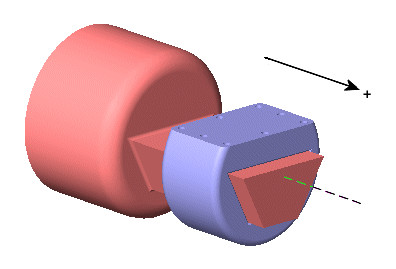
\includegraphics[width=.24\linewidth]{./intro/figures/prismaticJoint.jpg}} \hfill
    \subfloat[Articulation simple de type rotoïde]{\label{intro:fig0view1}
    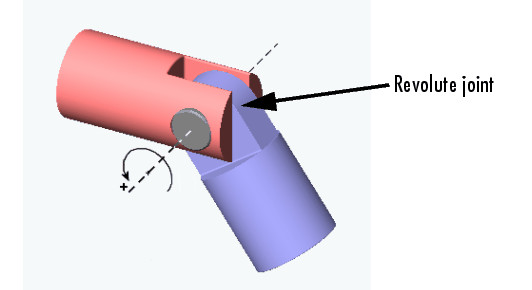
\includegraphics[width=.24\linewidth]{./intro/figures/revoluteJoint.jpg}} \hfill
  \subfloat[Articulation composée de type cylindrique]{\label{intro:fig0view2}
    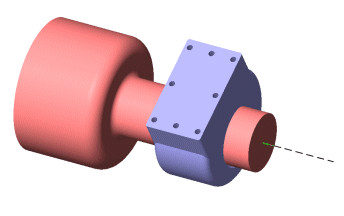
\includegraphics[width=.24\linewidth]{./intro/figures/cylindricalJoint.jpg}} \hfill
  \subfloat[Articulation composée de type sphérique]{\label{intro:fig0view3}
    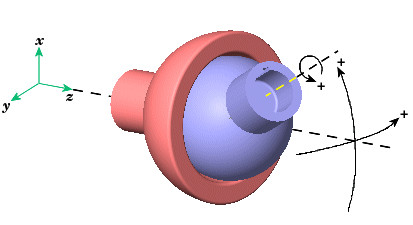
\includegraphics[width=.24\linewidth]{./intro/figures/sphericalJoint.jpg}}
    \caption{\footnotesize{Différents exemples d'articulations.}}
\label{intro:fig0}
\end{figure}

On appelle {\it coordonnées articulaires} l'ensemble des valeurs prises par les paramètres permettant de décrire l'état des articulations à un instant donné. Les coordonnées articulaires sont exprimées dans un espace articulaire propre à chaque articulation. Les paramètres nécessaires à l'expression des coordonnées articulaires sont généralement au nombre de 3 pour un point (ses coordonnées dans l'espace cartésien) et de 6 pour un solide (position cartésienne complétée par trois angles de rotation). Le nombre de paramètres non fixés par la géométrie du robot et nécessaires à la description exhaustive des coordonnées d'une articulation est appelé {\it degré de liberté}. Lorsque les articulations ne sont pas laissées libres, leur valeur dans l'{\it espace articulaire} sera contr\^olée par des {\it actionneurs} : on distinguera donc les {\it articulations actionnées} des {\it articulations passives}.

De la même manière, on parlera des {\it coordonnées opérationnelles} pour définir la pose de l'organe terminal, exprimées par rapport à un référentiel de référence. A nouveau, nous pouvons définir les degrés de liberté de l'organe terminal comme le nombre de paramètres contr\^olés pour le déplacer dans l'espace. Cette notion est à distinguer de la mobilité de l'organe terminal, qui correspond aux possibilités de déplacement de l'organe terminal, contrôlées ou laissées libres. Si l'on décide par exemple de contr\^oler les mouvements en translation, de bloquer deux rotations mais d'en laisser libre une, la mobilité sera de 4, mais le nombre de degrés de libertés ne sera que de 3.

Enfin, on peut définir pour chaque segment son {\it degré de connexion} comme étant le nombre de solides auxquels il est relié par une articulation libre ou actionnée. Lorsque l'ensemble des segments ont un degré de connexion égal à 2 à l'exception de la base et de l'organe terminal qui ont de degré de connexion égal à 1, on parle de {\it cha\^ine cinématique ouverte} (Fig.\ref{intro:fig1view0}). Lorsque l'un des segments au moins (différent de la base) possède un degré de connexion supérieur ou égal à 3, nous avons une {\it cha\^ine cinématique fermée} (Fig.\ref{intro:fig1view1}) \cite{journals/gosselin1989}. Les cha\^ines cinématiques complexes sont constituées de plusieurs cha\^ines fermées et/ou ouvertes.

\begin{figure}[!ht]
  \centering
      \subfloat[Schéma d'une cha\^ine cinématique ouverte]{\label{intro:fig1view0}
    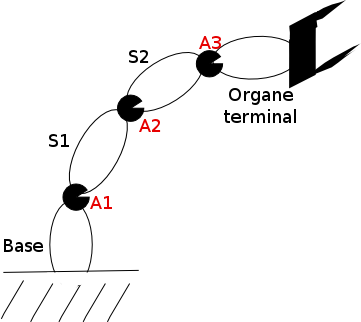
\includegraphics[width=.48\linewidth]{./intro/figures/openchain.png}} \hfill
    \subfloat[Schéma d'une cha\^ine cinématique fermée]{\label{intro:fig1view1}
    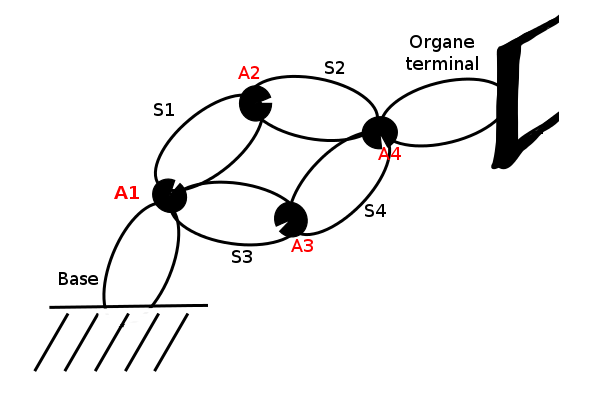
\includegraphics[width=.48\linewidth]{./intro/figures/closedchain.png}}
    \caption{\footnotesize{Exemples de cha\^ines cinématiques ouvertes et fermées : les $S_i$ représentent les différents segments intermédiaires, tandis que les $A_i$ correspondent aux articulations. Dans Fig.\ref{intro:fig1view0}, tous les segments $S_i$ ont un degré de connexion égal à 2 ; seuls la base et l'organe terminal ont un degré de connexion égal à 1. Il est visible dans Fig.\ref{intro:fig1view1} que tous les segments à l'exception de $S_4$ possèdent un degré de connexion ègal à 3.}}
\label{intro:fig1}
\end{figure}

\subsection{Architectures séries}

{\it On appelle robot série un système constitué d'une chaîne cinématique ouverte dont chaque segment est relié au suivant par une articulation simple} (Fig.\ref{intro:fig2}). Longtemps dominants dans l'industrie, les robots séries ont été privilégiés grâce à un erelative simplicité de la commande et un espace de travail important.

\begin{figure}[!ht]
  \centering
      \subfloat[Robot série présentant 3 articulations rotoïdes]{\label{intro:fig2view0}
    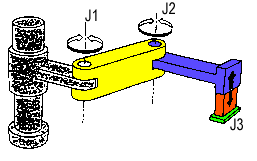
\includegraphics[width=.48\linewidth]{./intro/figures/serialrobot01.png}} \hfill
    \subfloat[Robot série présentant 3 articulations prismatiques]{\label{intro:fig2view1}
    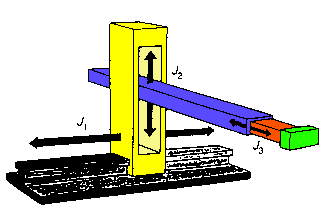
\includegraphics[width=.48\linewidth]{./intro/figures/serialrobot02.png}}
    \caption{\footnotesize{Exemples de robots séries}}
\label{intro:fig2}
\end{figure}

Une architecture série présente toutefois plusieurs inconvénients non négli\-gea\-bles dans un contexte industriel tels que :
\begin{itemize}
 \item chaque segment et articulation porte la charge de tous ceux qui leur succèdent dans la chaîne cinématique, ce qui pénalise la dynamique : segments et articulations doivent donc être rigidifiés et deviennent plus lourds, 
 \item les erreurs de positionnement se propagent de segments en segments ; la précision tout comme la répétabilité du manipulateur en sont affectées,
 \item les charges manipulables ne peuvent être excessives, car elles seront supportées par chacun des segments et articulations.
\end{itemize}

Ainsi, une architecture série impose souvent un dispositif imposant, dont la précision, la dynamique et la faible capacité de charges se révèleront insuffisants pour un grand nombre de tâches requises en particulier par l'industrie moderne.

Une alternative possible consiste en l'utilisation de chaînes cinématiques fermées permettant
\begin{itemize}
 \item une répartition des charges (segment ultérieurs et poids de l'objet manipulé),
 \item une compensation des erreurs entre chaque ``branche'' de la chaîne cinéma\-tique fermée,
 \item une plus grande rigidité des articulations, impliquant une dynamique plus grande.
\end{itemize}

Les architectures parallèles en particulier présentent une des déclinaisons possibles de chaînes cinématiques fermées, et leurs caractéristiques -- sur lesquel\-les nous allons nous pencher par la suite -- ont contribué à ce qu'elles s'installent progressivement dans le paysage de la robotique.


\subsection{Architectures parallèles}

Une définition des robots parallèles est donnée dans \cite{merlet1997robots} :\\
{\it Un manipulateur parallèle est constitué d’un organe terminal à $n$ degrés de li\-berté et d’une base fixe, reliés entre eux par au moins deux chaînes
cinématiques indépendantes, la motorisation s’effectuant par $n$ actionneurs simples.}\\

Parmi les exemples les plus cités dans la littérature, nous trouvons la plateforme de Gough-Stewart \cite{1956:Gough}, \cite{1965:Stewart} et le robot Delta \cite{1988:Clavel} (Fig.\ref{intro:fig3}).

Initialement développée pour des applications dans l'industrie automobile (Fig.\ref{intro:fig3view0}), la plateforme de Gough-Stewart a par la suite été utilisée dans des applications diverses parmi lesquelles les simulateurs de vols (Fig.\ref{intro:fig3view1}). Sa plateforme mobile peut être déplacée selon 6 degrés de liberté (3 translations $+$ 3 rotations) à l'aide de six jambes indépendantes actionnées par des vérins pneumatiques. Les articulations la reliant à la base (cardan) et à la plateforme (rotule) sont quant à elles laissées libres.

Le robot Delta (Fig.\ref{intro:fig3view2}) permet un déplacement de sa platforme selon les trois degrés de liberté de translation. Trois jambes sont utilisées pour cela, chacune étant reliée à la base par une articulation rotoïde à un levier, lui-même relié à un parallélogramme par une seconde articulation rotoïde, une troisième articulation rotoïde liant ce segment à l'organe terminal. Il peut atteindre des vitesses allant jusqu'à 10 m/s et des accélérations jusqu'à 20G, ce qui le rend particulièrement adapté pour des tâches de conditionnement. 

\begin{figure}[!ht]
  \centering
      \subfloat[Plateforme de Gough utilisée dans une usine de pneumatiques]{\label{intro:fig3view0}
    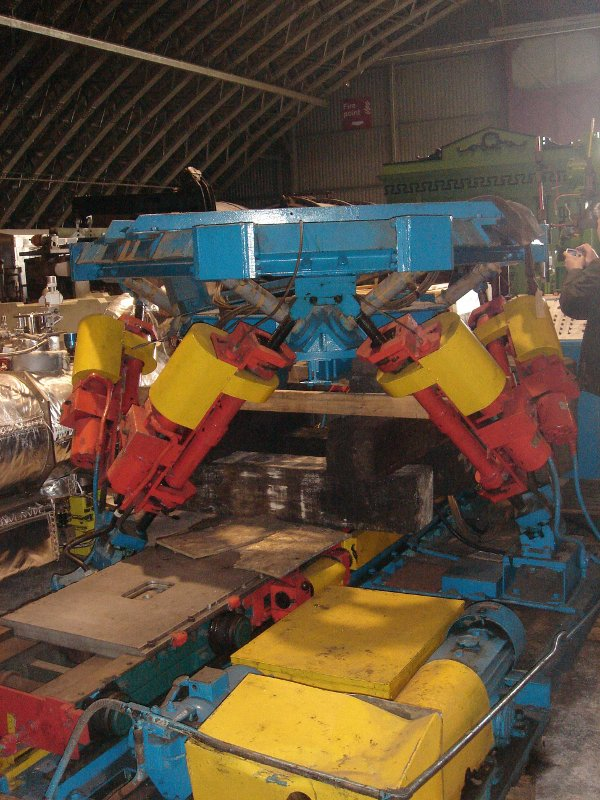
\includegraphics[width=.34\linewidth]{./intro/figures/parallelrobot01.jpg}} \hfill
    \subfloat[Plateforme de Gouch-Stewart utilisée pour des simulateurs de vols]{\label{intro:fig3view1}
    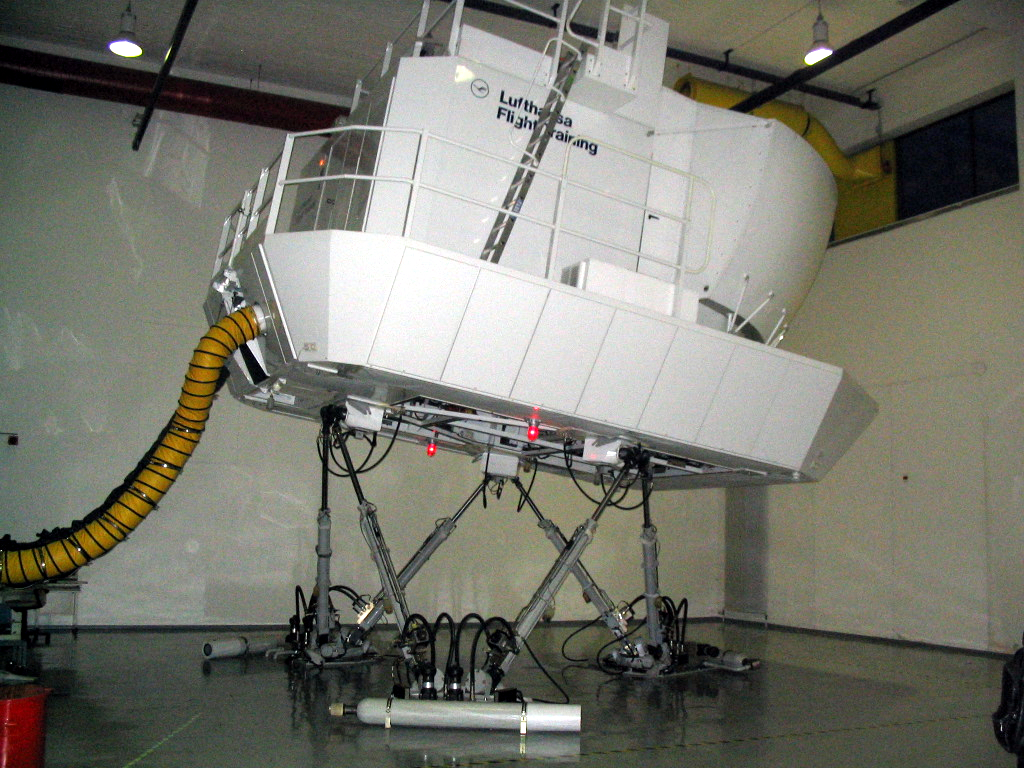
\includegraphics[width=.60\linewidth]{./intro/figures/parallelrobot02.jpg}} \\
    \subfloat[Robot Delta, particulièrement adapté aux tâches de conditionnement ou de ``pick and place'']{\label{intro:fig3view2}
    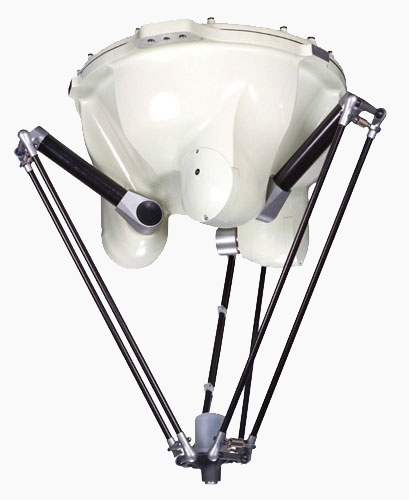
\includegraphics[width=.45\linewidth]{./intro/figures/parallelrobot03.jpg}}
    \caption{\footnotesize{Exemples de robots parallèles}}
\label{intro:fig3}
\end{figure}

De manière générale, les manipulateurs parallèles présentent les caractéristi\-ques sui\-vantes permettant de les comparer avantageusement aux manipulateurs séries :
\begin{itemize}
 \item une précision accrue par un mécanisme de {\bf compensation} des erreurs entre les différentes chaînes cinématiques (parfois appelées {\it jambes}),
 \item une capacité de charge élevée due à la {\bf répartition} de la charge sur les différentes jambes,
 \item une grande rigidité qui peut être élevée car les éléments de chaînes sont sollicités en traction/compression plutôt qu'en flexion.
 \item une dynamique élevée conséquente de la {\bf coopération} des différentes jam\-bes dans le positionnement de l'organe terminal.
\end{itemize}

Toutefois, les mécanismes parallèles possèdent plusieurs inconvénients qui doivent être pris en compte lors du choix d'une architecture :
\begin{itemize}
 \item des relations complexes entre entrées et sorties,
 \item des positions dites {\it singulières} pouvant conduire à une perte de contrôle du manipulateur, et qui limite l'espace de travail.
 \item un espace de travail restreint aux limites de variation des variables articulaires. A titre d'exemple, la variation d'altitude d'une plateforme de Gough-Stewart ne peut excéder la course des actionneurs linéaires des jambes.
\end{itemize}

L'architecture des robots parallèles à c\^ables que nous allons présenter dans la section suivante a été proposée dans le but de s'affranchir de cette dernière contrainte de limitation de l'espace de travail, qui est une contrainte forte des mécanismes parallèles.  L'intégralité des travaux présentés dans ce manuscrit étant consacré à l'étude et au développement de cette catégorie particulière de manipulateurs, nous utiliserons dorénavant pour les désigner les noms de robots, manipulateurs, robots parallèles à câbles ou CDPR (pour {\it cable-driven parallel robot}).

\section{Les manipulateurs parallèles à câbles}

Les manipulateurs parallèles à câbles présentent une structure en chaînes cinéma\-tiques fermées, la base et la plateforme étant reliées au moyen de câbles. Les actionneurs sont en général positionnés sur la base et leur fonction consiste à contrôler la longueur des câbles.

Afin de contrôler la longueur des câbles, plusieurs types de systèmes peuvent être utilisés, parmi lesquels :
\begin{itemize}
 \item un tambour actionné par un moteur rotatif sur lequel s'enroule ou se déroule le câble (Fig.\ref{intro:fig4view0}). La mesure de la longueur du câble déroulé est obtenue en mesurant la rotation du tambour ; cette mesure est relativement imprécise si l'enroulement n'est pas guidé.
 \item le câble est attaché au chariot d'un actionneur linéaire, un système de démultiplication à poulies permettant d'amplifier le déplacement du câble (Fig.\ref{intro:fig4view1}). La mesure du déplacement du chariot permet une estimation précise de la longueur du câble \cite{merlet2008}. 
\end{itemize}

\begin{figure}[!ht]
  \centering
      \subfloat[L'enroulement et le déroulement des câble se fait ici par un système de poulie actionnée par un moteur]{\label{intro:fig4view0}
    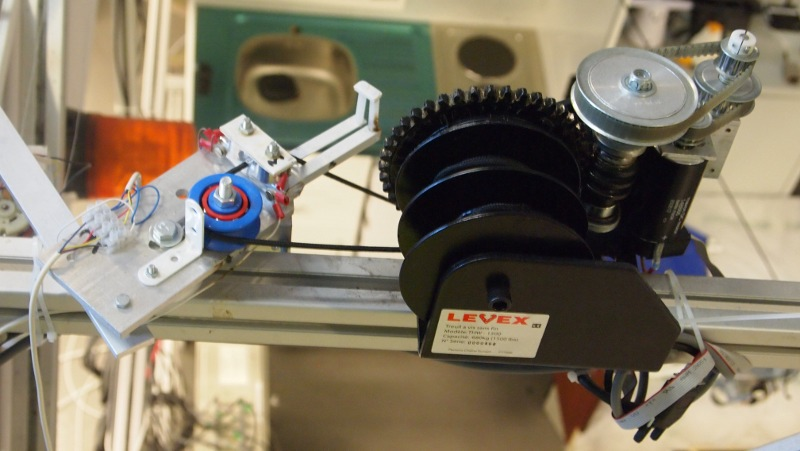
\includegraphics[width=.55\linewidth]{./intro/figures/winchesactuator.jpg}} \hfill
    \subfloat[Les câbles sont fixés à des plateformes pouvant se déplacer linéairement sur des rails, permettant un contrôle de la longueur]{\label{intro:fig4view1}
    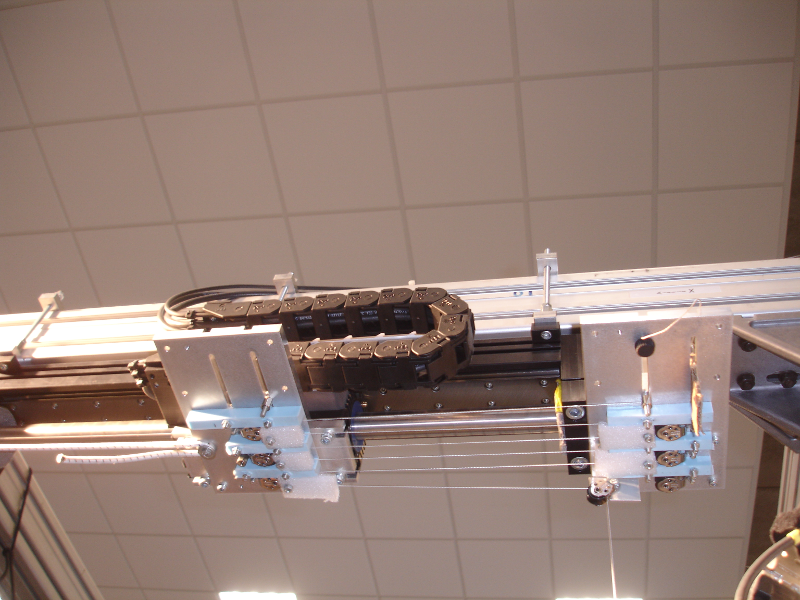
\includegraphics[width=.42\linewidth]{./intro/figures/linearactuator.png}}
    \caption{\footnotesize Deux types d'articulations et d'actionnement pour un robot à câble}
\label{intro:fig4}
\end{figure}

Dans tous les cas, ces systèmes permettent d'obtenir une trè large variation sur les longueurs des câbles, solutionnant ainsi le problème de l'espace de travail. On a pu ainsi construire des robots travaillant sur des volumes de $100m\times35m\times35m$ ({\tt Marionet-Crane}, Fig.\ref{intro:fig7view0}).

Toutefois, quelque-soit le type d'articulation et d'actionnement choisis, la force que peut exercer un seul câble sur l'organe terminal est nécessairement unilatérale : {\em un câble seul peut tirer, mais ne peut pas pousser la plateforme}. Il faut donc, pour pouvoir contrôler le mouvement dans son intégralité, que les câbles subissent une opposition. Il a ainsi été montré que $n+1$ câbles au minimum sont requis pour assurer le contrôle de $n$ degrés de liberté \cite{1994:Ming.Higuchi}. On peut cependant considérer la gravité comme une force unilatérale et la représenter comme un câble virtuel jouant le rôle d'opposition : il est ainsi possible de n'utiliser que $n$ câbles pour $n$ degrés de liberté.

On distingue donc deux types de configurations pour un robot parallèle à câbles :
\begin{itemize}
 \item en {\it configuration pleinement contrainte} (Fig.\ref{intro:fig5view0}), les câbles travaillent en opposition et $n+1$ sont nécessaires pour assurer des déplacements et l'application de forces correspondant à $n$ degrés de liberté.
 \item en {\it configuration suspendue} (Fig.\ref{intro:fig5view1}), la gravité agit comme un câble virtuel : les câbles sont fixés généralement au point le plus haut du dispositif, et $n$ suffisent pour déplacer et orienter l'organe terminal selon $n$ degrés de liberté. On retrouve parfois ce type de configuration dans la littérature sous le nom de {\it grue}/{\it crane}. Pour exemple, le manipulateur {\it Nist Spider} \cite{1992:Albus.Bostelman.ea} mentionné précédemment présente une configuration suspendue.
\end{itemize}

\begin{figure}[!ht]
  \centering
     \subfloat[Exemple de configuration pleinement contrainte]{\label{intro:fig5view0}
    
\includegraphics[width=.50\linewidth]{./intro/figures/robot_cdpr_noncrane.jpg}} \hfill
    \subfloat[Exemple de configuration suspendue]{\label{intro:fig5view1}
    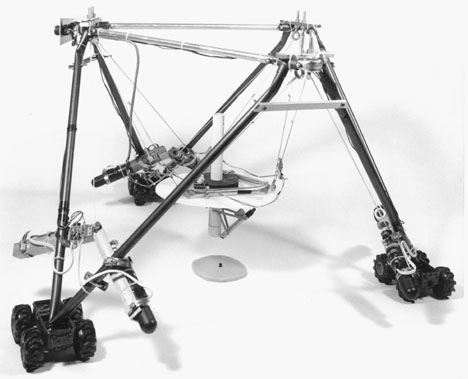
\includegraphics[width=.40\linewidth]{./intro/figures/robot_cdpr_crane.jpg}}
    \caption{\footnotesize Deux configurations possibles pour un robot parallèle à câble}
\label{intro:fig5}
\end{figure}

Une caractéristique particulière des manipulateurs parallèles à câbles qui les différencie des manipulateurs parallèles classiques est la {\bf non-rigidité des jam\-bes}. Sous certaines conditions, un ou plusieurs câbles peuvent être détendus, ce qui a pour effet qu'ils n'exercent plus de force sur la plateforme. Nous reviendrons plus loin sur ce point essentiel.

Comparativement donc aux robots parallèles classiques, les robots parallèles à câbles présentent les caractéristiques suivantes :
\begin{itemize}
 \item la structure parallèle permet de conserver les propriétés de compensation des erreurs, de répartition des charges et des efforts, de coopération des chaînes cinématique pour l'exécution d'un mouvement
 \item l'espace de travail est considérablement agrandipar rapport aux robots parallèles à jambes rigides
 \item l'équipage mobile est très léger, ce qui peut favoriser la dynamique
 \item le comportement des câbles (non-déformables, élastiques, pesants, \dots) peut complexifier le modèle du robot sérieusement
 \item l'unilatéralité des forces implique que nous puissions nous retrouver dans une situation avec un ou plusieurs câbles détendus, ce qui doit être pris en compte dans le contrôle.
\end{itemize}

Après avoir introduit quelques notations, nous allons à présent décrire les modèles géométriques direct et inverse, cinématiques ainsi que l'équilibre statique pour les robots parallèles à câble. Ceci nous permettra de lister tant que faire se peut l'ensemble des difficultés posées par ce type de manipulateur et auxquelles nous avons été confrontées dans le cadre de nos recherches.

\subsection{Notations}

\begin{figure}[!ht]
\centering
\def\svgwidth{.85\linewidth}
\input{./intro/figures/notation_schema.pdf_tex}
\end{figure}

\begin{itemize}
 \item $R_b$ : référentiel de la base
 \item $R_e$ : référentiel de l'organe terminal
 \item $A_i$ : point d'attache du $i^{\hbox{ème}}$ câble à la base ; le terme de {\it point de sortie} sera également utilisé.
 \item $B_i$ : point d'attache du $i^{\hbox{ème}}$ câble à l'organe terminal
 \item $C$ : un point arbitraire de l'organe terminal utilisé comme référence pour sa position
 \item $\rho_i$ : longueur réelle du câble $i$
 \item $l_i$ : longueur déroulée du câble $i$
 \item $\bf {\mathcal F}$ : vecteur des forces exercées sur l'organe terminal
 \item $\bf J$ : jacobienne du robot
\end{itemize}
Enfin, on utilisera la notation $J^{-1}$ pour exprimer la jacobienne inverse, et $J^{-T}$ sera utilisé comme raccourci de notation pour sa transposée.

Sauf mention du contraire, {\bf nous supposerons dans la suite que les câbles sont non-pesants et non-élastiques}, ce qui est une hypothèse adéquate pour le robot que nous avons utilisé.

\subsection{Modèle géométrique inverse}

Le modèle géométrique inverse consiste à déterminer les coordonnées articulaires à partir des coordonnées opérationnelles. Dans le cas des robots parallèles à câbles, les coordonnées articulaires correspondent aux longueurs $\rho$ des câbles. Lorsque ceux-ci sont tendus, cette longueur doit être égale à la distance entre les points de sortie ${\bf A}_i$ et le point d'attache à la plateforme ${\bf B}_i$. Dans le cas où le câble est détendu, la longueur sera supérieure à cette distance (Fig.\ref{intro:fig6view0}).\\

%%%%%% une figure différente
\begin{figure}[!ht]
  \centering
      \subfloat[Forme d'un câble dont la tension serait nulle]{\label{intro:fig6view0}
    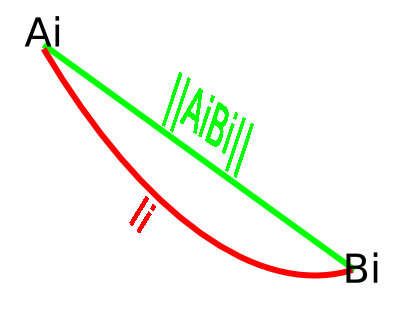
\includegraphics[width=.35\linewidth]{./intro/figures/nulltensionwire.png}} \hfill
    \subfloat[Câble élastique sur lequel est appliquée une tension positive : la longueur réelle diffère de la longueur déroulée]{\label{intro:fig6view1}
    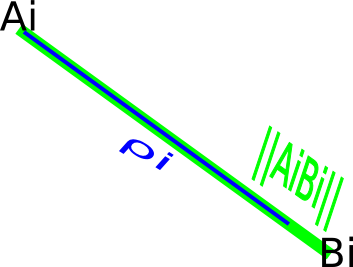
\includegraphics[width=.35\linewidth]{./intro/figures/positivetensionwire.png}} \\
    \caption{\footnotesize{Dans le cas d'un câble détendu (tension nulle), la longueur déroulée sera supérieure à la distance entre les deux points d'attache ; de plus, la forme du câble sera telle qu'il y a risque d'intersection avec d'autres câbles, l'environnement, \dots. Dans le cas d'un câble élastique tendu (tension strictement positive), la longueur déroulée sera inférieure à la distance entre les points d'attache correspondant à la longueur réelle du câble}}
\label{intro:fig6}
\end{figure}

Nous partons donc des relations suivantes :
\begin{eqnarray}
\rho_i &=& ||{\bf A}_i {\bf B}_i||, \hbox{ if } \tau_i > 0 \\ 
\rho_i &\geq& ||{\bf A}_i {\bf B}_i||, \hbox{ if } \tau_i = 0
\label{intro:eq1}
\end{eqnarray}

Comme on le voit, il n'est pas possible d'obtenir les longueurs $\rho_i$ sont prendre en compte les tensions $\tau_i$. Dès lors, tout comme dans l'approche développée par \cite{2010:Carricato.Merlet}, nous parlerons donc de modèle géométrico-statique inverse, requérant l'étude de l'équilibre statique.

\subsection{Equilibre statique}

On dit d'un solide au repos qu'il est en équilibre statique lorsque l'ensemble des forces extérieures $\mathcal {\bf F}_{\hbox{ext}_i}$ qui s'exercent sur lui s'annulent, ce qui se traduit par la relation suivante :
\begin{equation}
\sum_i \mathcal {\bf F}_{\hbox{ext}_i} = \vec {\bf 0}
\label{intro:eq2}
\end{equation}

Sous l'hypothèse que les forces mécaniques de frottement et de résistance peuvent être ici négligées, nous considérons uniquement la force de gravité exercée sur la plateforme ainsi que les efforts exercés par chacun des câbles.

La direction dans laquelle un câble de longueur $\rho_i$ relié à la base au point ${\bf A}_i$ et à la plateforme au point ${\bf B}_i$ exerce une force sur la plateforme est donnée par le vecteur ${\bf u}_i = \frac{{\bf A}_i{\bf B}_i}{\rho_i}$. On peut dès lors définir pour ce câble un torseur ${\bf W}_i$ correspondant aux efforts et couples exercés par celui-ci sur la plateforme :
\begin{equation}
{\bf W}_i = ({\bf u}_i^T, p_i \times {\bf u}_i)^T)^T
\label{intro:eq3}
\end{equation}
où $p_i$ est un vecteur allant d'un premier point de référence arbitraire localisé sur la plateforme à un second point placé sur le segment $[A_iB_i]$. La force exercée par le câble sur la plateforme est alors ${\bf W}_i \tau_i$ , où $\tau_i$ est un scalaire positif représentant l'intensité de la tension. De la même manière, en posant 


Soit ${\bf W}_g$ le torseur indiquant la direction dans laquelle la gravité est exercée dans le référentiel choisi, pour $n$ câbles, (Equ.\ref{intro:eq2}) s'écrit pour nous :
\begin{equation}
\begin{bmatrix}
 {\bf W}_1 & {\bf W}_2 & \dots & {\bf W}_n & {\bf W}_g
\end{bmatrix}
\begin{bmatrix}
 \tau_1 \\ \tau_2 \\ \dots \\ \tau_n \\ \hbox{mg}
\end{bmatrix}
= \vec {\bf 0}
\label{intro:eq4}
\end{equation}

En posant ${\bf \tau} = (\tau_1, \tau_2, \dots, \tau_n)^T$, ${\bf W}$ la matrice $6 \times n$ dont les colonnes sont les $n$ torseurs ${\bf W}_i$, et en isolant $\mathcal {\bf F} = {\bf W}_g \hbox{mg}$ modélisant la force de gravité, la relation (Equ.\ref{intro:eq4}) s'écrit également :
\begin{equation}
\mathcal {\bf F} + {\bf W} \tau = \vec {\bf 0}
\label{intro:eq5a}
\end{equation}

soit  
\begin{equation}
\mathcal {\bf F} = {\bf J}^{-T} {\bf \tau}
\label{intro:eq5b}
\end{equation}
où ${\bf J}^{-1} = - {\bf W}^T$ est une matrice que l'on appelle {\it jacobienne inverse}.

\subsection{Modèle géométrico-statique inverse (ou {\it MGSI})}

Connaissant les paramètres de pose de la plateforme, on peut en déduire les longueurs supposées $\rho_i$ des câbles à partir des données du modèle géométrique inverse. Dans le cas où nous avons $m \geq 6$ câbles, l'équilibre statique possède en théorie une infinité de solutions. Nous ne considérons alors que les ensembles de solutions pour lesquelles les $\rho_i$ sont tous strictement positifs. Si $m = 6$, la solution de l'équilibre statique est unique.

Il nous faut cependant étudier les situations pour lesquelles l'équilibre statique est vérifié pour $ m < 6$ câbles. Dans ce cas, si les $\tau_i$ correspondants sont strictement positifs, cela signifie qu'une solution existe avec seulement $m < 6$ câbles, et nous ne contrôlons plus que $m$ degrés de libertés.

Nous nous retrouvons dans une même situation lorsque nous étudions un CDPR sous-contraint, c'est-à-dire possédant moins de câbles que de degrés de libertés. Pour un robot à $m < 6$ câbles, l'équilibre statique est vérifié uniquement si l'ensemble des déterminants $m+1 \times m+1$ de la matrice ${\bf W}$ sont nuls \cite{carricato_merlet2013}. Si tous les $\tau_i$ sont strictement positifs, le modèle géométrico-statique possède alors une solution, mais correspondant à un mode dégradé du système.


\subsection{Modèle géométrico-statique direct}

Résoudre le modèle géométrique direct consiste à calculer les coordonnées opéra\-tionnelles à partir de la donnée des coordonnées articulaires. Il s'agit donc dans le contexte d'un robot parallèles à câbles de déduire la pose de la plateforme (position et orientation) à partir des longueurs des câbles. C'est un problème qui a posé de nombreux défis mathématiques et algorithmiques dans le cas des robots parallèles rigides \cite{merlet1997robots}.

Supposons que nous cherchions à déterminer l'ensemble des paramètres de pose (translations et rotations) pour un robot à $6$ câbles. Le {\it MGD} est alors un problème à $6$ variables. Si nous avons 6 (ou plus) câbles tendus, nous avons $6$ (ou plus) équations. La statique possède également $6$ variables (les tensions) et $6$ équations (les forces et couples dans chaque direction). On vérifie l'existence de l'équilibre avec la statique, puis nous pouvons déterminer l'ensemble des poses possibles pour les longueurs de câbles données.

Considérons maintenant que l'un des câbles est mou. Le {\it MGD} nous donne $5$ équations pour $6$ variables. La statique par contre nous donne $6$ équations (toujours les forces et couples exercés sur la plateforme) mais pour désormais $5$ variables (les $6-1$ câbles tendus). Nous nous retrouvons donc avec un système à $11$ équations contenant $11$ inconnues.

De manière générale, pour $p < 6$ câbles, nous aurons $p$ équations à $6$ inconnues fournies par le {\it MGD} et $6$ équations à $p$ inconnues grâce à l'équilibre statique. Soit $p+6$ équations à $6+p$ inconnues.

Supposons maintenant que notre manipulateur est en configuration suspendue avec $6$ câbles de longueurs connues. La résolution du système peut amener à une ou plusieurs solutions telle(s) que la tension dans les $6$ câbles est strictement positive. Si toutefois nous lançons la plateforme, avec des longueurs déroulées de câbles correspondant aux données du problème, il est possible qu'elle arrive à une des positions calculées, mais il est aussi possible qu'elle se retrouve dans une position complètement différente. En effet, la pose peut être telle qu'un ou plusieurs câbles ne seront pas tendus.

Si l'on veut résoudre le {\it MGD} pour un robot à câbles, l'ensemble suivant des situations doit donc être considéré, à savoir :
\begin{itemize}
 \item tous les câbles sont en tension, et il existe éventuellement plusieurs solutions
 \item un câble n'est pas en tension, le {\it MGD} doit être résolu pour $m-1$ câbles
 \item 2, 3, \dots câbles ne sont pas en tension, le {\it MGD} doit être résolu pour $m-2$, $m-3$, \dots câbles
\end{itemize}

Ce qu'il faut retenir ici, c'est qu'il est difficile lors d'un déplacement de prévoir à l'avance quels câbles seront en tension en chaque point de la trajectoire ainsi que la valeur des tensions.

Ce point, très peu mentionné dans la littérature, est un des inconvénients majeurs de l'utilisation des robots parallèles à câbles. Le premier chapitre de ce travail montrera qu'il est toutefois possible d'élaborer une stratégie prenant ce problème en compte pour améliorer le contrôle et la stabilité du système pour la grande majorité des situations.

\subsection{Modèle cinématique}

Le modèle cinématique consiste à établir une relation entre les vitesses des coordonnées articulaires ${\bf \Theta}$ et celles des coordonnées opérationnelles ${\bf X}$.

Nous avons vu que le vecteur ${\bf A}_i{\bf B}_i$ peut être calculé de deux manières différentes :
\begin{itemize}
 \item connaissant la pose de la plateforme et sa géométrie, les coordonnées de ${\bf B}_i$ sont données ; ${\bf A}_i$ étant connu par la géométrie du robot, on peut définir une fonction $H_1$ dépendante uniquement de la pose telle que :
\begin{equation}
{\bf A}_i{\bf B}_i = H_{1_{|i}}({\bf X})
\label{intro:eq6}
\end{equation}
 \item à partir des coordonnées articulaires (et éventuellement de la pose si l'intervention de l'équilibre statique est requise), le {\it MGSD} permet de définir la relation suivante :
\begin{equation}
{\bf A}_i{\bf B}_i = H_{2_{|i}}({\bf X}, {\bf \Theta})
\label{intro:eq7}
\end{equation}
\end{itemize}
 
Si ${\bf AB}$ est le vecteur composé des différents ${\bf A}_i{\bf B}_i$, alors on obtient en combinant (Equ.\ref{intro:eq6}) et (Equ.\ref{intro:eq7}) :
\begin{equation}
\begin{matrix}
{\bf AB} &=& H_1({\bf X}) \\
{\bf AB} &=& H_2({\bf X}, {\bf \Theta}) \\
\Longrightarrow & & H_1({\bf X}) = H_2({\bf X}, {\bf \Theta})
\end{matrix}
\label{intro:eq8}
\end{equation}

En différentiant (Equ.\ref{intro:eq8}), on obtient :
\begin{equation}
\frac{\partial H_1}{\partial {\bf X}} \frac{\partial {\bf X}}{\partial {\bf T}} =  \frac{\partial H_2}{\partial {\bf X}} \frac{\partial {\bf X}}{\partial {\bf T}} + \frac{\partial H_2}{\partial {\bf \Theta}} \frac{\partial {\bf \Theta}}{\partial {\bf T}}
\label{intro:eq9}
\end{equation}

soit :

\begin{equation}
\dot {\bf \Theta} = \left ( \frac{\partial H_2}{\partial {\bf \Theta}} \right )^{-1} \left (\frac{\partial H_1}{\partial {\bf X}} - \frac{\partial H_2}{\partial {\bf X}} \right ) \dot {\bf X}
\label{intro:eq10}
\end{equation}

Si $\left ( \frac{\partial H_2}{\partial {\bf \Theta}} \right )$ est bien inversible, nous pouvons définir une matrice $J^{-1}$ de manière à obtenir la relation suivante :
\begin{equation}
\dot {\bf \Theta} = J^{-1} \dot {\bf X}
\label{intro:eq11}
\end{equation}

Le vecteur $\dot {\bf X}$ est alors appelé le torseur cinématique et correspond à la variation instantanée des paramètres de pose par rapport au temps. La matrice $J^{-1}$  est également appelée {\it Jacobienne inverse} du robot, et dépend à la fois des paramètres de pose et des coordonnées articulaires.


\section{Présentation du {\tt Marionet-Assist}}

Les {\tt Marionet} sont une classe de robots à câbles développés par l'EPI Hephaistos pour des applications diverses :
\begin{itemize}
 \item {\tt Marionet-Crane} (Fig.\ref{intro:fig7view0}) : intervention à grande échelle pour des opé\-rations de sauvetage dans des situations de catastrophe naturelle
 \item {\tt Marionet-Rehab} (Fig.\ref{intro:fig7view1}) : rééducation et assistance à la personne ; pouvant atteindre des vitesses allant jusqu'à 100m/s, il est également possible de l'utiliser pour des opérations de transfert ultra-rapides
 \item {\tt Marionet-School} (Fig.\ref{intro:fig7view2}) : pédagogie et diffusion ; ces robots sont utilisés entre autres pour illustrer de manière ludique des propriétés géométriques et mathématiques auprès des publics jeunes
\end{itemize}

\begin{figure}[!ht]
  \centering
    \subfloat[{\tt Marionet-Crane} description]{\label{intro:fig7view0}
    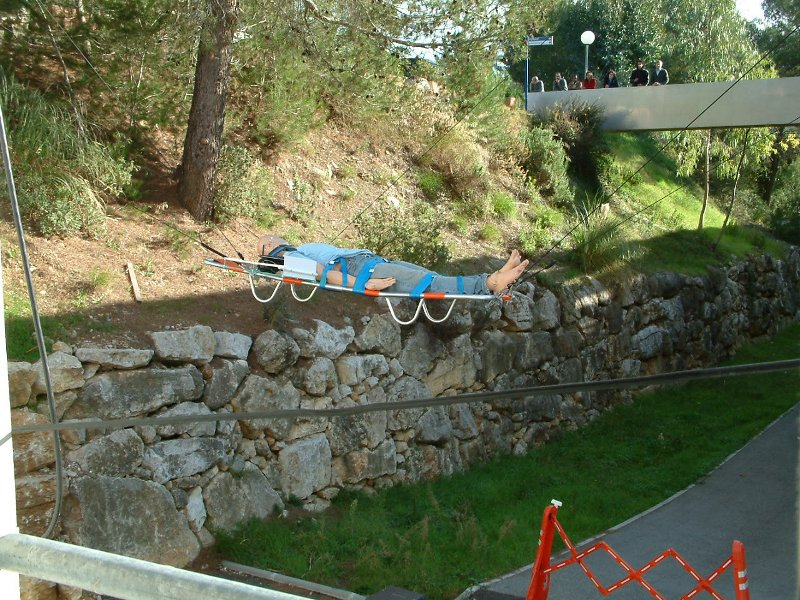
\includegraphics[width=.90\linewidth]{./intro/figures/marionet03.jpg}} \\
    \subfloat[{\tt Marionet-Rehab} description]{\label{intro:fig7view1}
    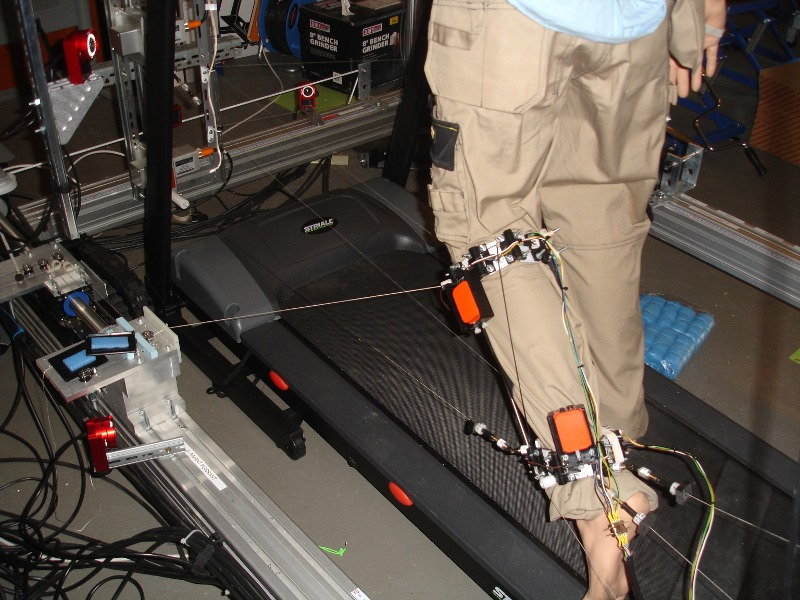
\includegraphics[width=.45\linewidth]{./intro/figures/marionet01.jpg}} \hfill
    \subfloat[{\tt Marionet-School} description]{\label{intro:fig7view2}
    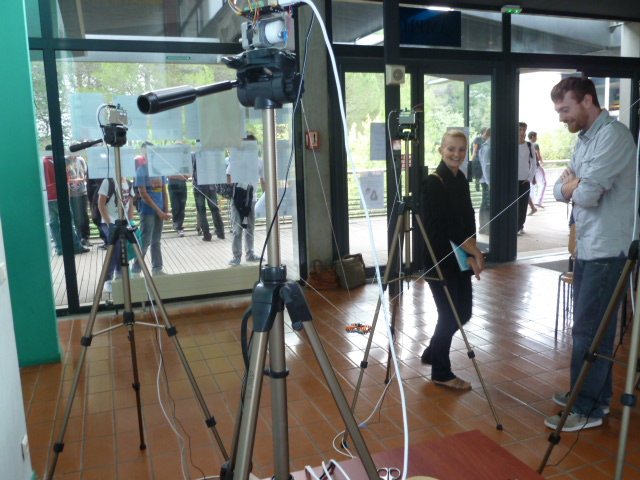
\includegraphics[width=.45\linewidth]{./intro/figures/marionet02.jpg}}
    \caption{\footnotesize{Exemples d'utilisation des robots {\tt Marionet}}}
\label{intro:fig7}
\end{figure}

Le robot {\tt Marionet-Assist} a été développé dans un objectif d'assistance aux personnes à mobilités réduites, et plus spécifiquement dans une démarche d'amélio\-ration de l'autonomie des publics concernés. Il doit pouvoir répondre à des situations tout aussi diverses que :
\begin{itemize}
 \item soutien ponctuelle au déplacement pour une personne âgée expérimentant une fatigue articulaire (par exemple pour la passage de la baignoire) (Fig.\ref{intro:fig8view0})
 \item aide au transfert d'une position à une autre pour une personne atteinte de paraplégie (des toilettes au fauteuil par exemple) (Fig.\ref{intro:fig8view1})
 \item soutien des aidants lors du transfert de personnes atteintes de tétraplégie (déplacement du lit vers un fauteuil par exemple) (Fig.\ref{intro:fig8view2})
\end{itemize}

\begin{figure}[htp]
  \centering
  \subfloat[Simple soutien au déplacement dans une pièce de vie]{\label{intro:fig8view0}
  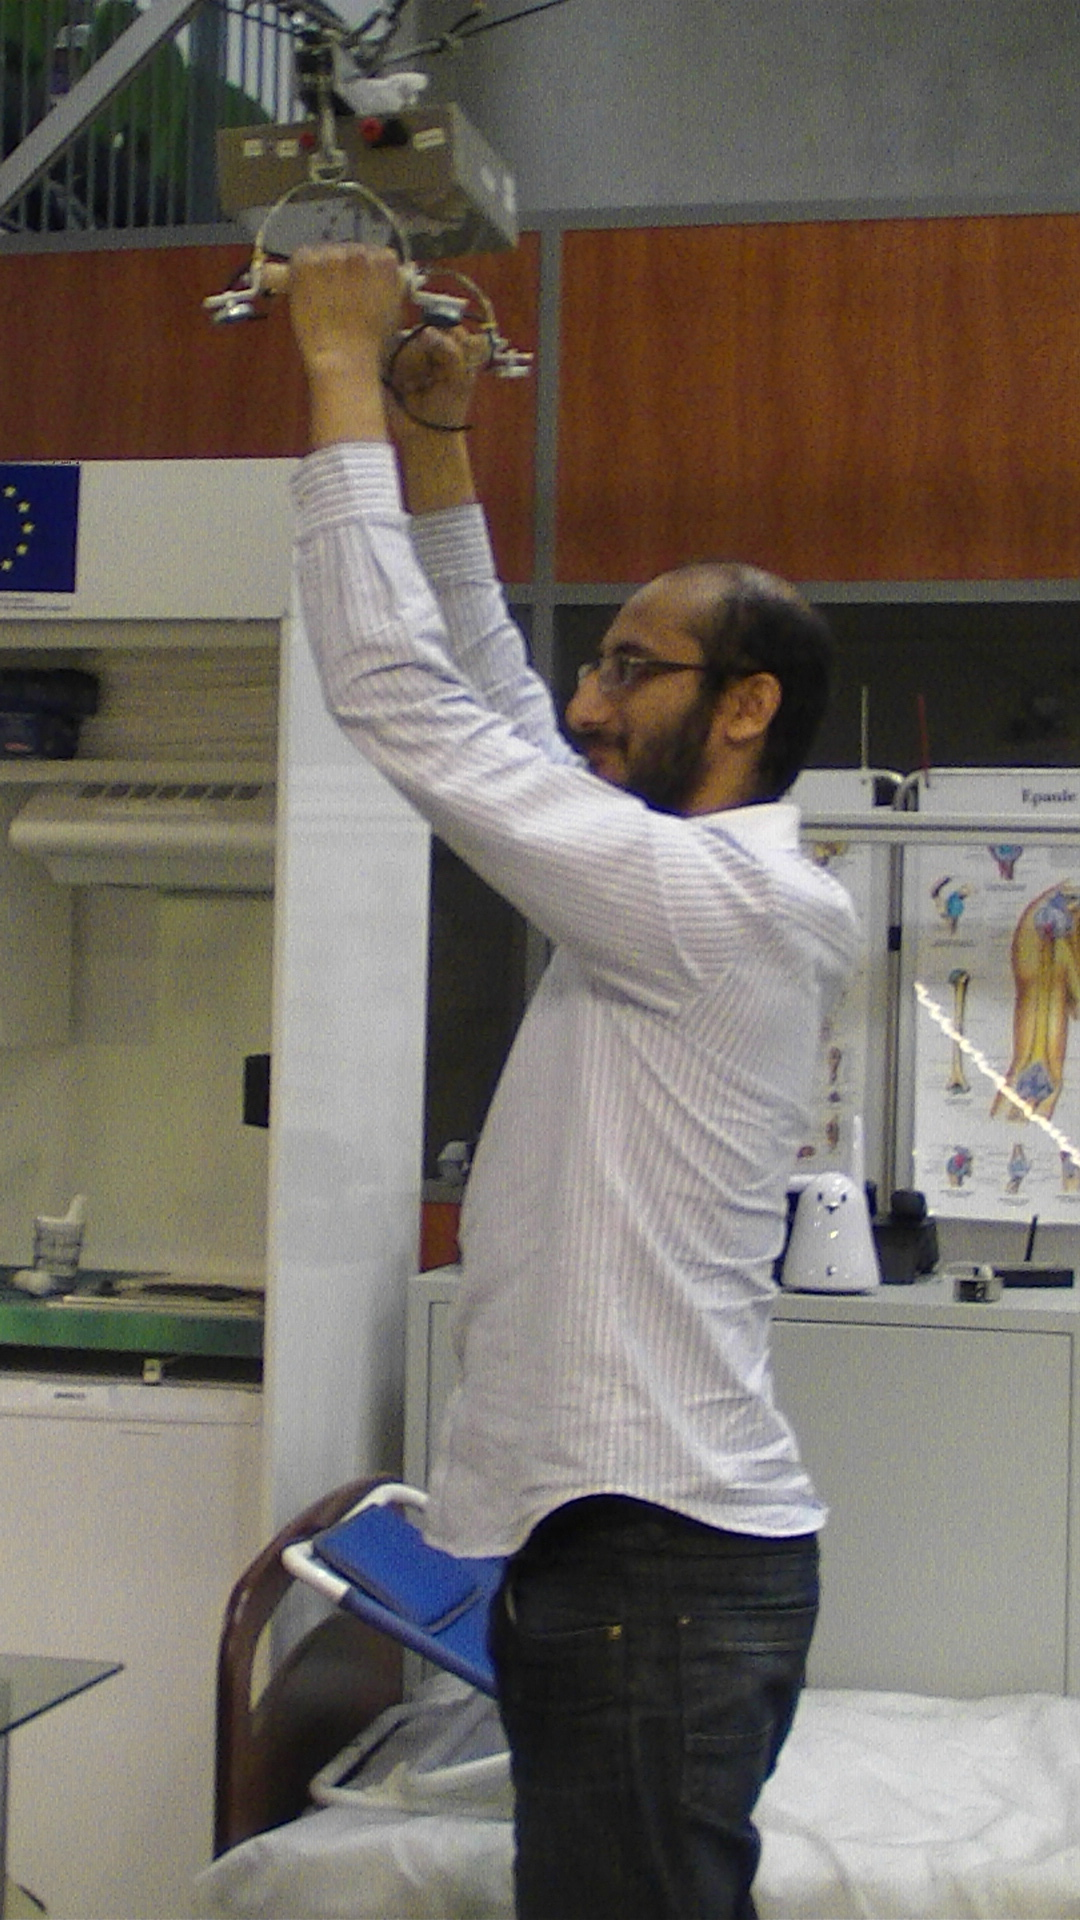
\includegraphics[width=.2\linewidth]{./intro/figures/case01.jpg}} \hfill
  \subfloat[Transfert de position assise/levé]{\label{intro:fig8view1}
  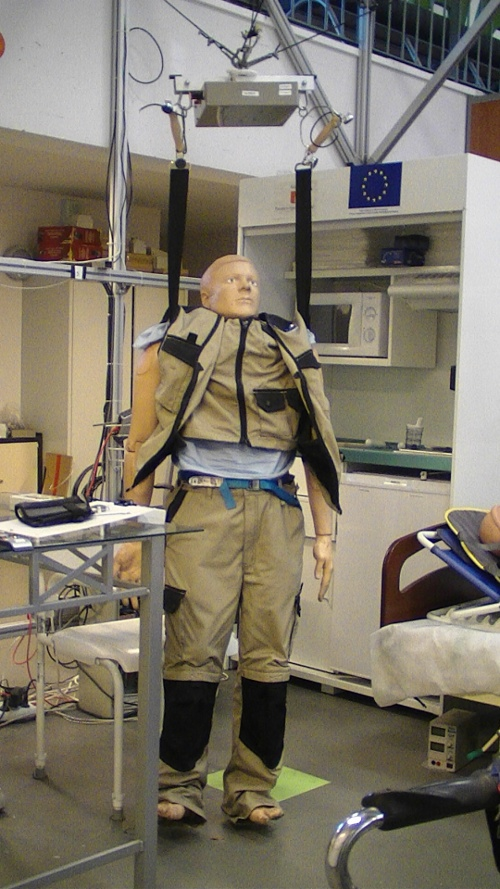
\includegraphics[width=.2\linewidth]{./intro/figures/case02.jpg}} \hfill
  \subfloat[Déplacement autonome d'un lieu de vie (lit) vers un dispositif de déplacement (fauteuil)]{\label{intro:fig8view2}
  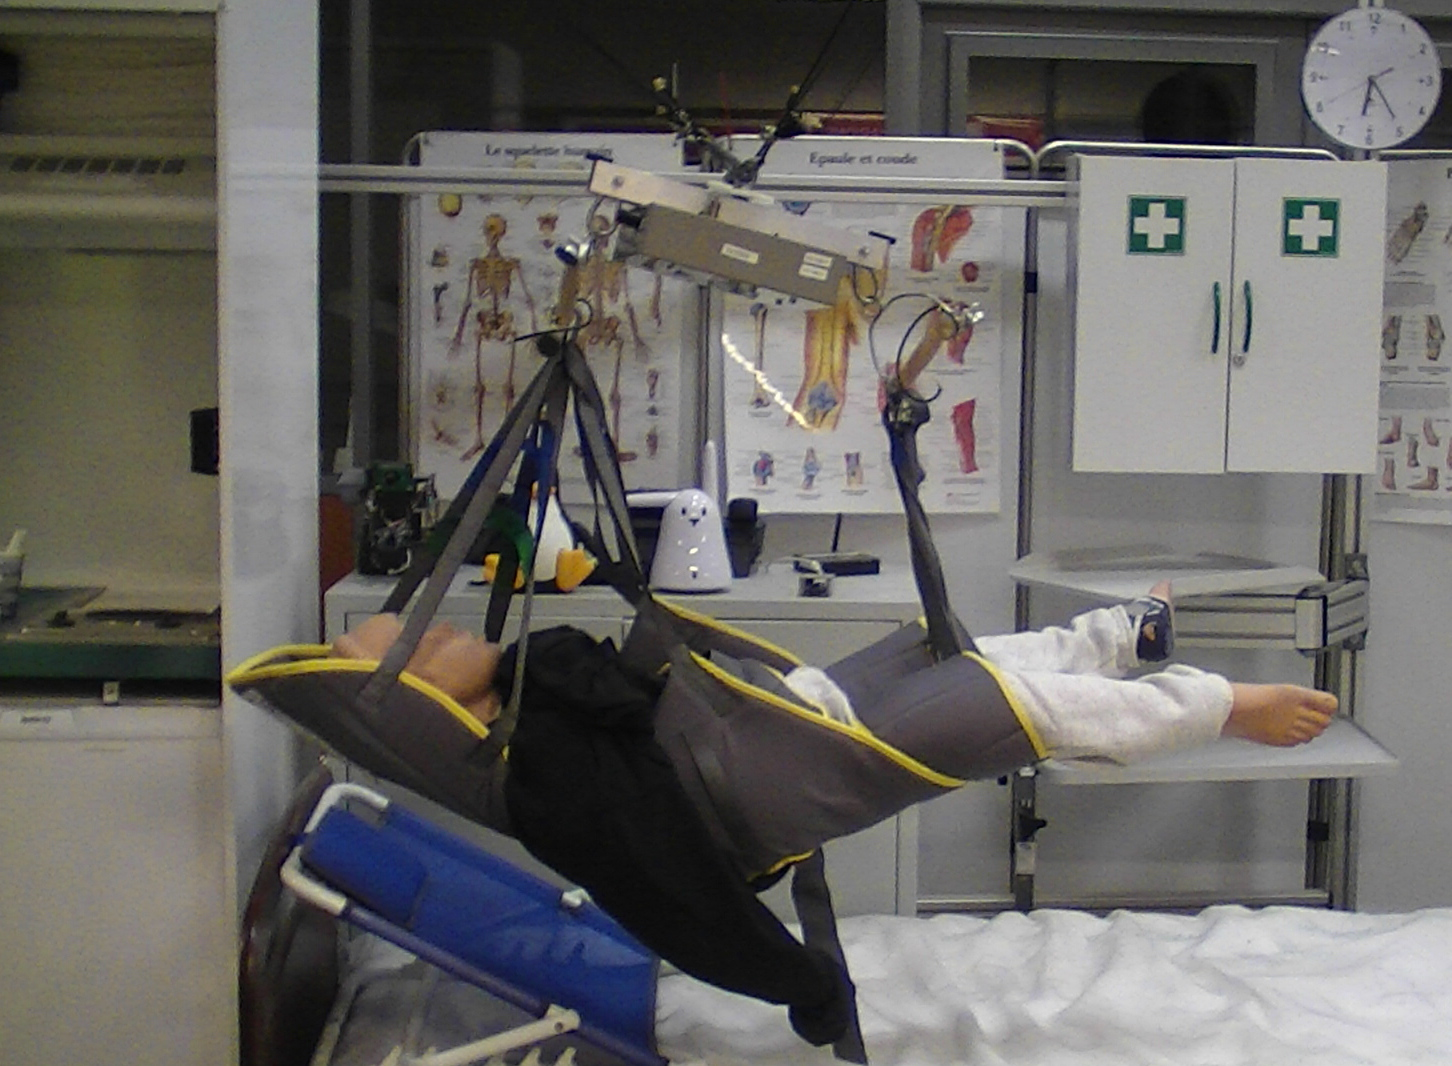
\includegraphics[width=.48\linewidth]{./intro/figures/case03.jpg}} \hfill
    \caption{\footnotesize{Différents types de fragilités motrices dans des situation de la vie quotidienne}}
\label{intro:fig8}
\end{figure}

Un dispositif répondant à ces impératifs doit présenter les caractéristiques suivantes :
\begin{itemize}
 \item pouvoir supporter des charges correspondant au poids d'une personne
 \item avoir un espace de travail équivalent à la taille d'une pièce de vie
 \item être léger et suffisamment discret et modulaire pour ne pas bouleverser l'environnement de l'utilisateur
 \item avoir une précision suffisante pour permettre un positionnement garantissant la sécurité, l'efficacité et le confort des opérations de transfert et d'attachement/détachement de l'utilisateur à la plateforme.
\end{itemize}

Le choix d'utilisation d'un robot parallèle à câbles semble donc le plus compatible avec l'ensemble de ces exigences. {\tt Marionet-Assist} a ainsi été conçu et déployé dans un appartement-témoin (Fig.\ref{intro:fig10view0},\ref{intro:fig10view1}) situé dans les locaux d'INRIA. Les câbles permettant le contrôle de la plateforme sont fixés sur le plafond de l'appartement. Dans sa configuration actuelle, {\tt Marionet-Assist} est équipé de $4$ câbles, mais peut en contrôler jusqu'à $6$. Plusieurs stratégies sont envisageables au niveau des points de fixation sur la plateforme :
\begin{itemize}
 \item les points d'attaches des câbles sont tous différents, il est alors possible avec $n$ câbles de contrôler $n$ degrés de liberté. Cette configuration sera notée $N-N$ (Fig.\ref{intro:fig9view0}).
 \item les câbles sont attachés en un même point à la plateforme : il est posible à partir de $3$ câbles de contrôler les déplacement en translation de la plateforme ; l'utilisation de plus de $3$ câbles permet alors d'augmenter la taille de l'espace de travail. On parle dans ce cas de configuration $N-1$ (Fig.\ref{intro:fig9view1}).
 \item certains câbles seulement sont attachés en un même point sur la plateforme. Dans le cas par exemple d'une disposition pour laquelle $3$ câbles sont atttachés en un même point $B_0$ et un quatrième câble relié à la plateforme en un point $B_1$, cette configuration sera notée $4-3-1$ (Fig.\ref{intro:fig9view2}).
\end{itemize}

\begin{figure}[htp]
  \centering
  \subfloat[Configuration $4-4$ : chaque câble est relié à la plateforme en un point distinct]{\label{intro:fig9view0}
  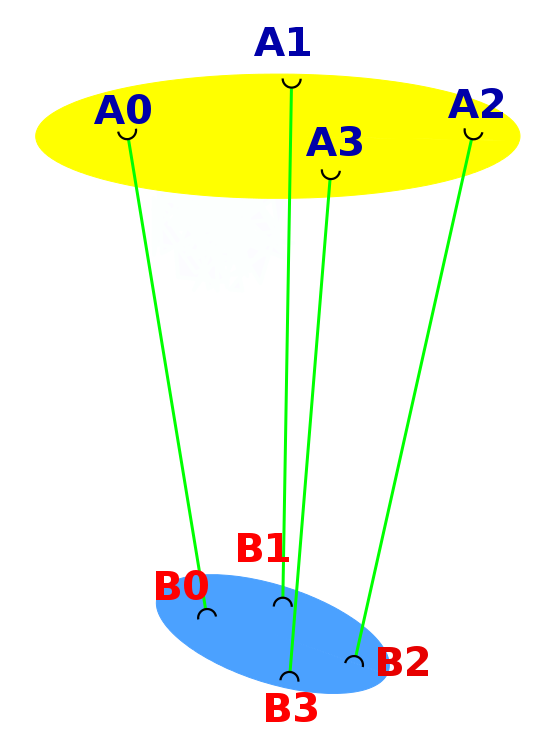
\includegraphics[width=.3\linewidth]{./intro/figures/cfg_44.png}} \hfill
  \subfloat[Configuration 4-1 : Les $4$ câbles sont reliés à la plateforme un un seul point]{\label{intro:fig9view1}
  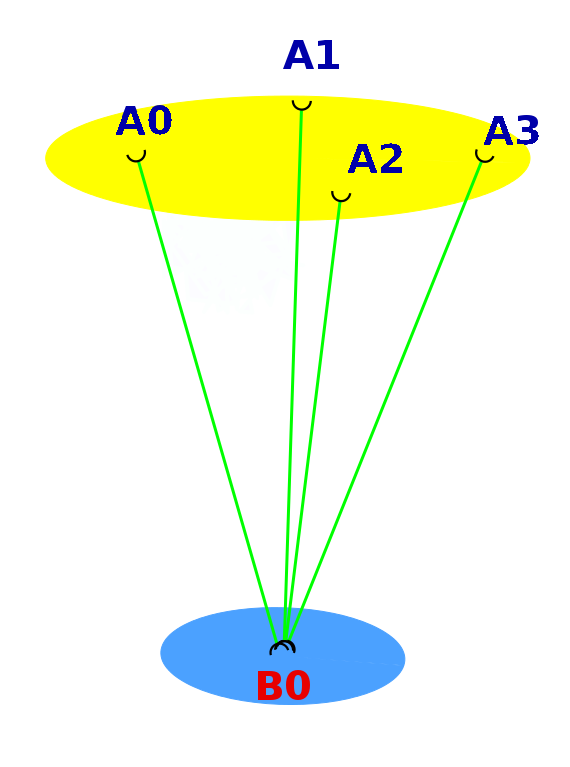
\includegraphics[width=.3\linewidth]{./intro/figures/cfg_41.png}}
  \subfloat[Configuration 4-3-1 : $3$ câbles sont reliés à la plateforme en un même point, le quatrième est relié en un point distinct]{\label{intro:fig9view2}
  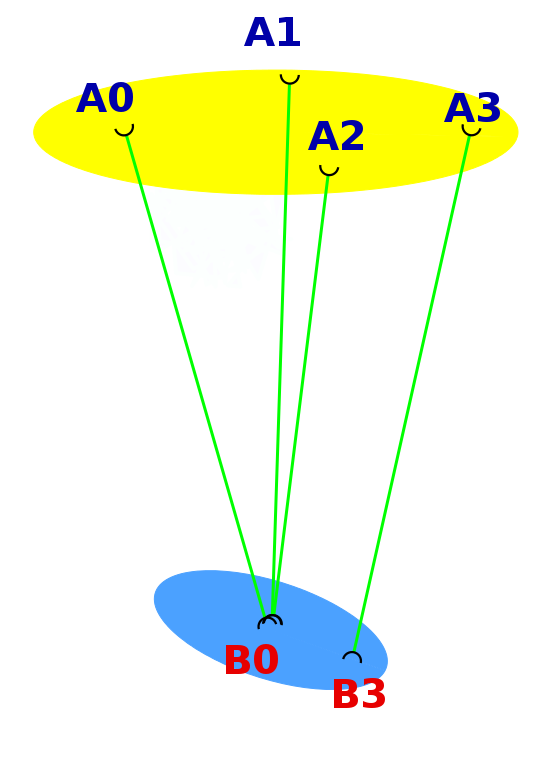
\includegraphics[width=.3\linewidth]{./intro/figures/cfg_431.png}} \hfill
    \caption{\footnotesize{Exemples de configurations avec $4$ câbles}}
\label{intro:fig9}
\end{figure}

Pour l'ensemble des expériences menées dans le cadre de ce travail, nous avons utilisé la configuration $4-1$ (Fig.\ref{intro:fig10view2}) qui nous permet de contrôler les déplacements en translation, le quatrième ayant été ajouté pour augmenter l'espace de travail de manière à pouvoir se déplacer dans la quasi-totalité de l'appartement-témoin. La figure (Fig.\ref{intro:fig11}) montre l'espace de travail atteignable pour chaque triplet de câbles en tension : on note qu'en tout point qui ne se trouve pas sur l'une des deux diagonales définies par les points $(A_0-A_2)$ et $(A_1-A_3)$, il existe pour chaque pose deux configurations possibles avec trois câbles en tension, et qu'à l'exception du point d'intersection de ces diagonales, au moins une configuration avec trois câbles tendus existe.

\begin{figure}[!ht]
\centering
\def\svgwidth{.90\linewidth}
\input{./intro/figures/MA_corobots.pdf_tex}
\caption{\footnotesize{La figure au centre représente le robot {\tt Marionet-Assist} ; en bas à gauche est représenté l'espace de travail atteignable lorsque les câbles attachés aux points $A_0$, $A_1$, $A_3$ sont en tension, en bas à droite l'espace de travail atteignable pour les câbles reliés aux points $A_0$, $A_1$, $A_2$. En haut à gauche, nous avons l'espace de travail correspondant aux câbles $A_0$, $A_2$, $A_3$ en tension, et en haut à droite l'espace de travail atteignable pour les câbles attachés aux points $A_1$, $A_2$, $A_3$.}}
\label{intro:fig11}
\end{figure}

Les câbles sont en Kevlar, ce qui nous permet de négliger leur élasticité et de pouvoir les modéliser comme des jambes rigides lorsque leur tension est strictement positive. Le contrôle des longueurs se fait à l'aide de poulies actionnées par des moteurs rotatifs (Fig.\ref{intro:fig10view3}). Toutefois, en l'absence de guide pour l'enroulement, il existe des incertitudes sur la longueur déroulée ; afin de pallier à cet inconvénient, des référentiels ont été disposés sur les câbles à intervalles connus, ce qui permet lors de leur détection de réactualiser la valeur estimée de la longueur déroulée.

\begin{figure}[htp]
  \centering
  \subfloat[Vue globale de l'appartement-témoin]{\label{intro:fig10view0}
  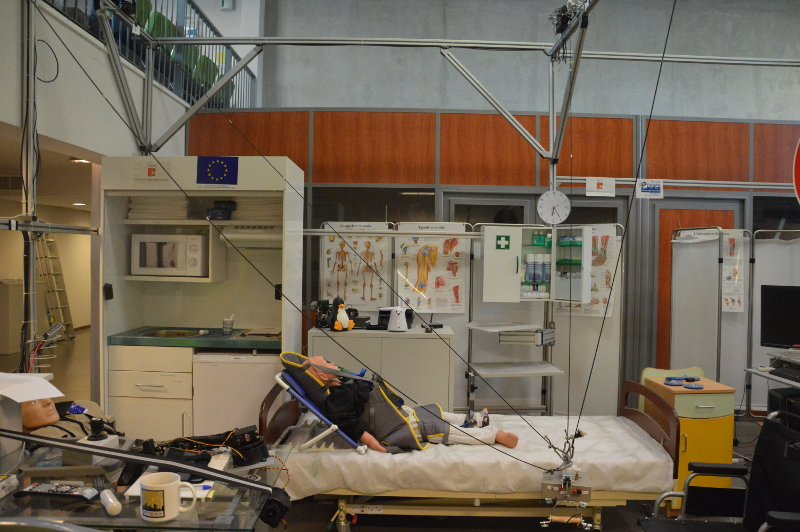
\includegraphics[width=.7\linewidth]{./intro/figures/view_appartment01.jpg}} \\
  \subfloat[Vue aérienne de l'appartement-témoin]{\label{intro:fig10view1}
  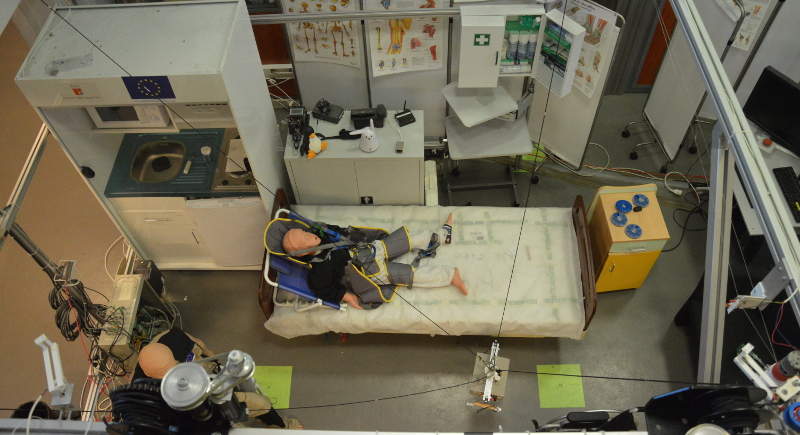
\includegraphics[width=.7\linewidth]{./intro/figures/view_appartment04.jpg}} \\
  \subfloat[Plateforme de {\tt Marionet-Assist}]{\label{intro:fig10view2}
  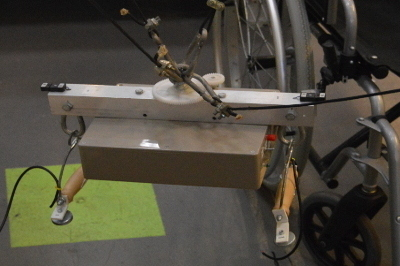
\includegraphics[width=.7\linewidth]{./intro/figures/view_plateform.jpg}} \\
  \subfloat[Système d'enroulement et actionneurs pour un câble]{\label{intro:fig10view3}
  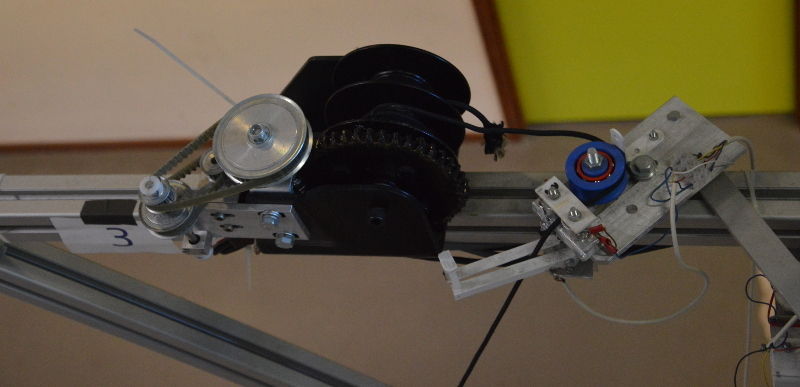
\includegraphics[width=.7\linewidth]{./intro/figures/view_winches02.jpg}}
    \caption{\footnotesize{{\tt Marionet-Assist}}}
\label{intro:fig10}
\end{figure}

Dans cette configuration, nous ne contrôlons que les trois degrés de liberté correspondant aux translations le long des axes du référentiel global. Pour un triplet de trois câbles en tension strictement positive, la solution au {\it MGD} est unique et peut être calculée analytiquement. La {\it Jacobienne inverse} possède en outre une forme relativement simple : ses lignes correspondent aux vecteurs $s = A_iB_i$ normalisés par la longueur $\rho_i$

\begin{equation}
{\bf J}^{-1}_i =
\begin{bmatrix}
 \frac {s_x} {\rho_i} & \frac {s_y} {\rho_i} & \frac {s_z} {\rho_i}
\end{bmatrix}
\label{intro:eq11}
\end{equation}

Ces propriétés font de {\tt Marionet-Assist} un robot adapté au contexte pour lequel il a été conçu. Nous avons cependant souhaité améliorer ses fonctionnalités de manipulation en lui permettant de ne pas seulement déplacer une personne, mais également des objets de la vie quotidienne. Il peut s'agir par exemple de ramasser un objet tombé au sol, ou d'amener à l'utilisateur un objet (des lunettes par exemple) localisé à un endroit de la pièce éloigné de celui auquel il se trouve. Afin de localiser l'objet, puis de guider le robot dans son déplacement et dans la manipulation de l'objet cible, une caméra a été ajoutée sur la plateforme, de manière à utiliser des techniques d'asservissement visuel. Ce sont ces dernières que nous allons à présent introduire, avant d'indiquer d'une part les problématiques posées par leur utilisation dans ce contexte particulier, et d'autre part les différentes possibilités d'améliorations que cela autorise concernant le contrôle des robots parallèles à câbles.

\section{Asservissement visuel}

 La vision représente pour les humains environ 70\% des données issues des perceptions sensorielles externes \cite{no} : d'une richesse incroyable, c'est aussi, par conséquent, une source d'erreurs inépuisable. La vision artificielle ne déroge pas à ses deux principes, d'où l'importance du traitement du signal d'une part (dans le but de recueillir et interpréter dans cette immensité d'informations ce qui est pertinent pour une tâche prescrite) et d'une stratégie d'asservissement d'autre part (afin de stabiliser une commande de tâche malgré les erreurs et incertitudes sur les données). Nous allons donc dans un premier temps présenter le mode d'acquisition des images, puis nous continuerons sur les modèles de perception utilisés. Une fois que nous aurons détaillé la manière dont une scène est projetée sur une image, nous pourrons distinguer plusieurs configurations et exposer différentes stratégies d'asservissement pouvant être utilisées. Nous développerons enfin les caractéristiques spécifiques à celle que nous avons sélectionnée dans le contexte de ces travaux.
 
 \subsection{Modèles de capteurs et projections}
 
 \subsubsection{De l'oeil à la caméra}
 
 Sans pour autant chercher à imiter la vision humaine, la vision artificielle s'en inspire néanmoins fortement pour ce qui concerne l'acquisition d'une scène. Ainsi, pour une caméra, le diaphragme joue le rôle de l'iris et de la pupille et détermine la quantité de lumière qui pourra être enregistrée sur un intervalle de temps donné. Par la suite, la lentille joue un rôle équivalent à la cornée et au cristallin, en faisant converger les rayons lumineux vers la rétine sur laquelle sont disséminés environ 125 millions de photorécepteurs : c'est au niveau de ces derniers que l'acquisition est véritablement effectuée. On distingue parmi les photorécepteurs :
 \begin{figure}[htp]
  \centering
  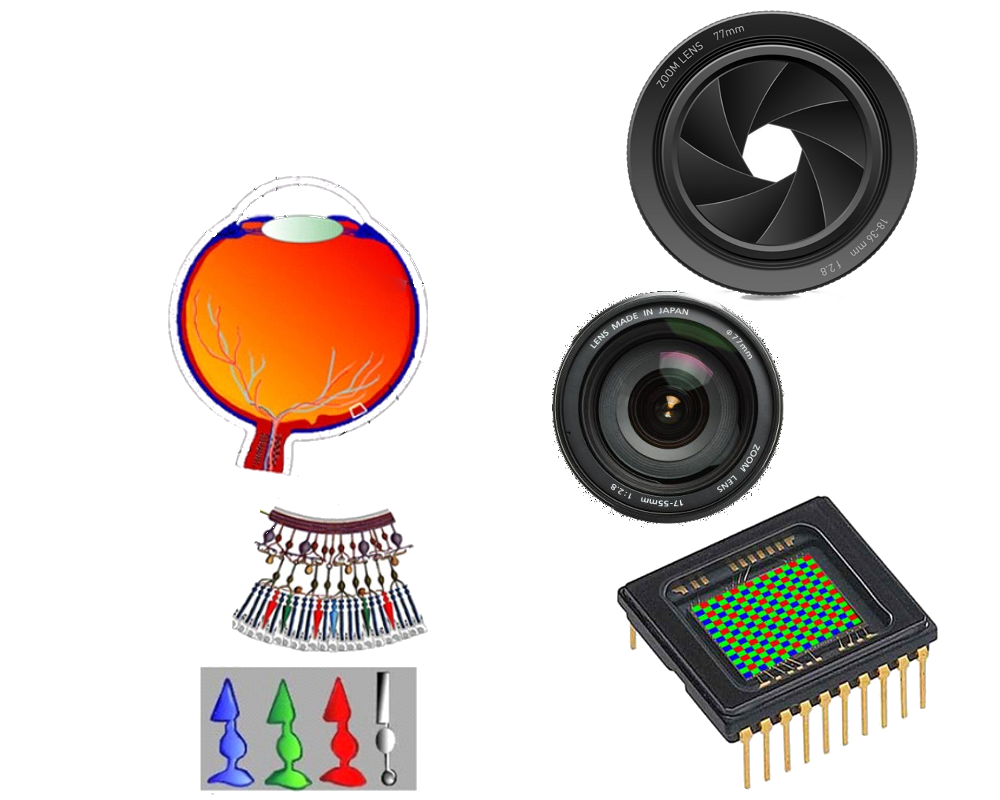
\includegraphics[width=.85\linewidth]{./intro/figures/oeil.png}
    \caption{\footnotesize{Oeil humain vs vision artificielle}}
\label{intro:fig11}
\end{figure}

 \begin{itemize}
  \item les cônes, généralement impliqués dans la vision diurne. Les cônes présentent 3 types de pigments leur permettant de réagir à des longueurs d'ondes spécifiques (qui ne recouvrent pas exactement le triplet RGB traditionnellement utilisé traitement d'image)
  \item les bâtonnets, impliqués dans la vision nocturne. Ne possédant d'un seul type de pigments, ils ne peuvent pas discriminer les longueurs d'ondes. En revanche, ils sont en moyenne 1000 fois plus sensibles à la lumière que les cônes, et leur population correspond à 20 fois celle des cônes.
 \end{itemize}

 Afin de simuler l'activité des photorécepteurs de l'oeil humain, les dispositifs technologiques les plus récents adoptent des stratégies basées sur l'utilisation de filtres placés en amont des capteurs photosensibles, permettant ainsi une acquisition en séquence (un même récepteur recevra successivement les réponses des filtres correspondants aux longueurs d'ondes distinguées) ou simultanée (les réponses sont envoyées sur des capteurs photosensibles dédiés).
  
L'information contenue dans les données ainsi recueillies est riche et multiple : elle peut-être de nature colorimétrique, géométrique, elle permet de ca\-ractériser des déplacements, des déformations. Toutefois, ce qui est vu n'est jamais qu'une représentation de ce qui est observé : il est donc nécessaire de reconstruire le plus fidèlement possible la scène initiale projetée sur les capteurs.
 
\subsubsection{De la scène à l'image}
 
Nous avons privilégié le modèle {\it pinhole} qui offre une approximation fiable des caméras perspectives (telles que celles que nous avons utilisées) tout en restant formellement simple\cite{Faugeras:1993}, sous les hypothèses du respect des conditions de Gauss (angles de faibles incidences), et -- c'est notre cas -- d'une absence de distorsion de la caméra.

Soient ${\bf P} = (X, Y, Z)$ les coordonnées 3-D d'un point dans l'espace et ${\bf p} = (x, y)$ ses coordonnées dans l'image. Le modèle de projection perspective consiste en une projection centrale de centre $\mathcal C$, portée par l'axe ${\bf z}_c$ représentant l'axe optique de la caméra. On appelle {\it plan image} le plan se trouvant à distance focale $f$ de la caméra, soit $Z = f$. On définit également un point de référence ${\bf c}(x_c,y_c)$ dans le plan image comme étant le point d'intersection de l'axe optique et du plan image (Fig.\ref{intro:fig12}).

\begin{figure}[h!tp]
  \centering
  \def\svgwidth{.95\linewidth}
  \input{./intro/figures/modele_projection.pdf_tex}
    \caption{\footnotesize{Modèle de projection {\it pinhole}}}
\label{intro:fig12}
\end{figure}

En plus du {\it référentiel-base} (pour rappel, noté, $\mathcal R_b$), s'ajoutent un {\it référentiel-caméra} noté $\mathcal R_c$, un {\it référentiel-objet} $\mathcal R_o$, ainsi qu'un {\it référentiel-image} $\mathcal R_i$. Nous noterons également $l_x$ et $l_y$ respectivement la longueur et la hauteur d'un pixel dont nous aurons besoin pour la suite.

A partir des coordonnées d'un point ${\bf P}(X, Y, Z)$ exprimées dans le référentiel de la caméra, les coordonnées projetées sur le plan images sont déduites de la manière suivante :

\begin{equation}
x = f \frac{X}{Z}, y = f \frac{Y}{Z}
\label{intro:eq12}
\end{equation}

ou, sous forme matricielle :

\begin{equation}
Z
\begin{bmatrix}
x \\y \\ 1
\end{bmatrix}
=
\begin{bmatrix}
f & 0 & 0 \\ 0 & f & 0 \\ 0 & 0 & 1 
\end{bmatrix}
\begin{bmatrix}
X \\ Y \\ Z 
\end{bmatrix}
\label{intro:eq13}
\end{equation}
soit $\widetilde {\bf p} = {\bf A}{\bf P}$, avec $\widetilde {\bf p} = Z {\bf p}$.

Un point dans l'image est généralement représenté par ses coordonnées pi\-xelliques (l'origine du référentiel étant supposée localisée en haut à gauche de l'image).

La conversion entre les coordonnées métriques $(x, y)$ et les coordonnées pixelliques $(x_p, y_p)$, se fait selon la relation suivante :

\begin{equation}
\left \lbrace
\begin{matrix}
x_p = x_c + x/l_x \\
y_p = y_c + y/l_y
\end{matrix} \right .
\label{intro:eq14}
\end{equation}
ce qui donne sous une forme matricielle :

\begin{equation}
\begin{bmatrix}
x_p \\y_p \\ 1
\end{bmatrix}
=
\begin{bmatrix}
\frac 1 {l_x} & 0 & x_c \\ 0 & \frac 1 {l_y} & y_c \\ 0 & 0 & 1 
\end{bmatrix}
\begin{bmatrix}
x \\ y \\ 1
\end{bmatrix}
\label{intro:eq15}
\end{equation}
soit ${\bf p}_p = {\bf B} {\bf p}$.

On obtient la relation suivante entre les coordonnées métriques 3-D du point et les coordonnées pixelliques dans l'image :
\begin{equation}
Z\begin{bmatrix}
x_p \\y_p \\ 1
\end{bmatrix}
=
\begin{bmatrix}
\alpha_x & 0 & x_c \\ 0 & \alpha_y & y_c \\ 0 & 0 & 1 
\end{bmatrix}
\begin{bmatrix}
X \\ Y \\ Z
\end{bmatrix}
\label{intro:eq16}
\end{equation}
avec $\alpha_x = f/l_x$ et $\alpha_y = f/l_y$. Les paramètres $(\alpha_x, \alpha_y, x_c, y_x)$ de la matrice $K = AB$ ainsi construite sont généralement obtenus par calibration. La matrice $K$ nous permet de faire le lien entre les informations géométriques disponibles dans l'image et la projection de la scène observée. En particulier, nous pouvons à présent définir les coordonnées normalisées ainsi :
\begin{equation}
\left \lbrace
\begin{matrix}
x = X/Z \\
y = Y/Z
\end{matrix} \right .
\label{intro:eq17}
\end{equation}
indépendantes de la focale, et pouvant être déduites des coordonnées pixelliques en utilisant la matrice $K$.

Il nous reste à établir une relation entre le référentiel-caméra et le référentiel-objet afin d'établir une correspondance entre les propriétés de la scène réelle et sa projection dans l'image. Pour cela, il suffit de déterminer les paramètres du changement de référentiel.

Soient ${}^c{\bf P} = ({}^cX, {}^cY, {}^cZ)$ les coordonnées du point ${\bf P}$ exprimées dans le référentiel $\mathcal R_c$ et ${}^o{\bf P} = ({}^oX, {}^oY, {}^oZ)$ ses coordonnées dans le référentiel $\mathcal R_o$. Le passage d'un référentiel à l'autre est effectué en utilisant la relation ${}^c{\bf P} = {}^c{\bf t}_o + {}^c{\bf R}_o {}^o{\bf P}$, avec ${}^c{\bf t}_o$ le vecteur $3\times 1$ de translation entre les deux référentiels, ${}^c{\bf R}_o$ la matrice $3\times 3$ de rotation correspondant à la rotation des axes du référentiel. En utilisant les coordonnées homogènes $\widetilde {\bf P}$ de ${\bf P}$, il est possible de factoriser cette transformation en une seule opération matricielle :
\begin{equation}
{}^c \widetilde {\bf P} = {}^c {\bf M}_o {}^o \widetilde {\bf P}
\label{intro:eq18}
\end{equation}
soit :
\begin{equation}
\begin{bmatrix}
{}^cX \\ {}^cY \\ {}^cZ \\ 1
\end{bmatrix}
=
\begin{bmatrix}
&  {}^c{\bf R}_o & & {}^c{\bf t}_o \\
& {\bf 0} & & 1
\end{bmatrix}
\begin{bmatrix}
{}^oX \\ {}^oY \\ {}^oZ \\ 1
\end{bmatrix}
\label{intro:eq19}
\end{equation}

On appelle ${}^c{\bf M}_o$ la {\it matrice homogène de transformation} du référentiel $\mathcal R_o$ au référentiel $\mathcal R_c$, dont l'inverse s'exprime simplement sous la forme :
\begin{equation}
{}^o{\bf M}_c = 
\begin{bmatrix}
&  {}^c{\bf R}_o^T & & -{}^c{\bf R}_o^T {}^c{\bf t}_o \\
& {\bf 0} & & 1
\end{bmatrix}
\label{intro:eq20}
\end{equation}

Nous sommes dès lors en mesure d'établir une relation entre les propriétés de la scène observée exprimées dans son référentiel propre et sa projection dans l'image, exprimée en coordonnées pixelliques, métriques et généralisées. Le lecteur remarquera cependant que, s'il est possible directement, connaissant ${\bf K}$ et ${}^o{\bf M}_c$, de déduire à partir des propriétés de la scène les caractéristiques de sa projection, l'opération inverse est dépendante dans ce modèle d'une estimation pour chaque point de sa coordonnée ${}^cZ$, ce que nous aurons à considérer plus tard.

\subsection{Configurations et stratégies d'asservissement visuel}

\subsubsection{Positionnement de la caméra}

Nous ne considérons dans la suite que l'utilisation d'une caméra unique dans le cas d'une scène fixe. Le contexte étant celui d'un manipulateur dont on veut asservir la saisie et le déplacement d'un objet, plusieurs stratégies s'offrent à nous. Une première décision à prendre concerne par exemple le positionnement de la caméra. On distingue ainsi une configuration déportée (Fig.\ref{intro:fig13view0}) d'une configuration embarquée (Fig. \ref{intro:fig13view1}).

\begin{figure}[htp]
  \centering
  \subfloat[La caméra est déportée ; la scène comprend l'organe terminal et l'objet-cible]{\label{intro:fig13view0}
    \def\svgwidth{.45\linewidth}
  \input{./intro/figures/eye_to_hand.pdf_tex}} \hfill
    \subfloat[La caéméra est embarquée ; la scène ne comprend que l'objet-cible]{\label{intro:fig13view1}
    \def\svgwidth{.45\linewidth}
  \input{./intro/figures/eye_in_hand.pdf_tex}} 
    \caption{\footnotesize{Positionnements de caméra}}
\label{intro:fig13}
\end{figure}

Dans le cas d'une caméra déportée, on connait les transformations permettant de passer du référentiel-base $\mathcal R_b$ au référentiel-caméra $\mathcal R_c$, et du référentiel-caméra au référentiel-objet $\mathcal R_o$. Seul l'organe terminal bouge dans la scène observée. Dans le cas d'une caméra embarquée, la transformation permettant de passer du référentiel de l'organe terminal $\mathcal R_e$ au référentiel-caméra $\mathcal R_c$ est connue. Toutefois, l'ensemble de la scène est affecté lors d'un déplacement de l'organe terminal (et donc de la caméra).

\subsubsection{Asservissements en position, basés images et hybrides}

De manière générale, une stratégie d'asservissement visuel peut être décomposée de la manière suivante :
\begin{enumerate}
 \item on sélectionne dans un premier temps un ensemble ${\bf s}$ de paramètres à partir desquels on peut estimer soit directement la pose de l'organe terminal, soit le déplacement nécessaire à l'obtention de cette pose. L'ensemble des paramètres dépend d'une part de la valeur des primitives extraites de l'image et d'autre part d'un ensemble de connaissances {\it a priori}, telles que les propriétés de la caméra, ou encore un modèle de la cible.
 \item on définit ensuite la valeur désirée ${\bf s}^*$ des paramètres, correspondant à l'état que l'on souhaite atteindre.
 \item à partir de données extraites de l'image, on calcule la valeur courante des paramètres
 \item on calcule alors une erreur ${\bf e} = {\bf s} - {\bf s}^*$, dont on souhaite qu'elle converge vers $0$.
 \item on établit enfin une relation entre la variation $\dot {\bf e}$ de l'erreur et la commande qui sera ensuite envoyée au manipulateur.
 \item la commande est effectuée, et l'on boucle les étapes $3$ à $6$ jusqu'à obtention d'une valeur seuil de l'écart entre les valeurs courantes des paramètres et les valeurs désirées.
\end{enumerate}

\begin{figure}[htp]
  \centering
    \def\svgwidth{.95\linewidth}
  \input{./intro/figures/bloc_commande.pdf_tex}
    \caption{\footnotesize{Schéma des étapes de l'asservissement visuel}}
\label{intro:fig13}
\end{figure}

On distinguera ici deux grandes classes de stratégies d'asservissement : la première est basée sur l'estimation des paramètres de pose de l'organe terminal (PBVS : position-based visual servo), tandis que la seconde utilise directement les primitives extraites de l'image (IBPS : image-based visual servo). Il est également possible de mixer ces deux approches, ce que l'on appellera un asservissement hybride.

Dans le cas de l'asservissement en position, une connaissance du modèle 3-D de la cible est nécessaire (on parle d'ailleurs parfois d'asservissement 3-D). De l'écart entre les valeurs courantes d'un ensemble de primitives et leurs valeurs estimées pour une pose désirée, on déduira les paramètres de pose de l'organe terminal. Cela revient à faire varier un référentiel courant de l'organe terminal $\mathcal R_e$ vers un référentiel correspondant à la pose prescrite $\mathcal R_e^*$, soit la détermination d'une matrice homogène de transformation ${}^{e^*}{\bf M}_e$. Comme nous l'avons vu, cette matrice est composée d'une translation et d'une rotation, qui peuvent être décrites à l'aide de $6$ paramètres. Dans ce cas, le vecteur ${\bf s}$ est constitué de mesures permettant de construire cette matrice de transformation de repère. On pourra d'ailleurs noter que dans une configuration avec caméra embarquée, le problème est équivalent à la détermination d'une matrice de transformation ${}^{c^*}{\bf M}_c$ entre les référentiels courants et désirés de la caméra.

L'asservissement basé-image repose quant à lui sur l'exploitation direct des informations extraites de l'image pour établir la commande qui sera envoyée au manipulateur. Il ne nécessite pas de connaissance {\it a priori} du modèle 3-D de l'objet, mais exploite des primitives pour lesquelles on possède un modèle de comportement lorsqu'elles évoluent dans l'espace. On parlera dès lors d'asser\-vissement 2-D, ou d'asservissement 2-D 1/2 lorsque une connaissance du modèle 3-D est néanmoins utilisée (approche hybride).

Quelque-soit la situation, l'objectif de l'asservissement visuel est de traduire un ensemble de mesures effectuées dans une série d'image en loi de commande qui sera envoyée au manipulateur.

\subsubsection{Construction d'une loi de commande}

Nous reprenons ici les bases de construction d'une loi de commande. Le lecteur les retrouvera développées par exemple dans \cite{chaumette:tuto01} et \cite{chaumette:tuto02}. Nous nous contentons ici d'exposer les principes généraux d'outils que nous avons utilisés tout au long de nos travaux.

Soient ${\bf s}$ un ensemble de mesures réalisées au sein de l'image sur des primitives choisies, et ${\bf s}^*$ les valeurs désirées de ces mesures. On construit le vecteur ${\bf e} = {\bf s} - {\bf s}^*$ représentant l'erreur de mesure, soit la différence entre les valeurs courantes et les valeurs désirées.

On choisit ici de construire une loi de commande en vitesse. Soit le torseur cinématique ${\bf v}_c = ({\bf \nu}_c, {\bf \omega}_c)$, avec ${\bf \nu}_c$ et ${\bf \omega}_c$ les vitesses instantanées respectivement linéaires et angulaires. Il est nécessaire dans un premier temps de déterminer les variations $\dot {\bf s}$ des mesures pour un déplacement donné ${\bf v}_c$ de la caméra. Cette relation, lorsqu'elle existe, prend la forme algébrique d'une matrice ${\bf L}_s \in \mathcal M_{k\times 6}$ que l'on appelle {\it matrice d'interaction}, $k$ représentant le nombres de mesures effectuées. A partir de tous ces éléments nous pouvons établir :

\begin{equation}
\dot {\bf s} = {\bf L}_s {\bf v}_c
\label{intro:eq21}
\end{equation}

Notre cible étant fixe, nous avons $\dot {\bf e} = \dot {\bf s}$. Nous pouvons dès lors immédiatement déduire de (Equ.\ref{intro:eq21}) la relation suivante :
\begin{equation}
\dot {\bf e} = {\bf L}_e {\bf v}_c
\label{intro:eq22}
\end{equation}

Nous souhaitons que notre erreur ${\bf e}$ de mesure décroisse de manière exponentielle, soit : $\dot {\bf e} = - \lambda {\bf e}$, $\lambda$ étant appelé le {\it gain}, permettant de régler la vitesse de convergence. La loi de commande suivante peut alors être construite :
\begin{equation}
{\bf v}_c = - \lambda {\bf L}_e^+ {\bf e} 
\label{intro:eq23}
\end{equation}
où ${\bf L}_e^+ \in \mathcal M_{6 \times k}$ représente la matrice pseudo-inverse de Moore-Penrose, soit ${\bf L}_e^+ = ({\bf L}_e^T {\bf L}_e)^{-1} {\bf L}_e^T$. Lorsque $k = 6$ et que $\det {\bf L}_e \neq 0$, on pourra choisir d'utiliser la loi ${\bf v}_c = - \lambda {\bf L}_e^{-1} {\bf e} $.

En pratique, il est difficile de connaître avec exactitude ${\bf L}_e$, qui peut être dépendante de la pose de la caméra. On utilisera dès lors une approximation de la matrice d'interaction, la loi de commande finale devenant :
\begin{equation}
{\bf v}_c = - \lambda \widehat {{\bf L}_e^+} {\bf e} 
\label{intro:eq23}
\end{equation}

Toutes les fois où cela est possible, on préfèrera utiliser des primitives dont la matrice d'interaction correspondante exhibe des propriétés algébriques inté\-ressantes (triangulaire, inversible, \dots). Le choix préalable des primitives obéit donc à un double impératif :
\begin{itemize}
 \item on attend qu'elles soient aisément identifiables dans l'image et que les mesures puissent être réalisées de manière robuste
 \item les caractéristiques de la matrice d'interaction qu'elles complètent doivent comporter des qualités algébriques qui permettront d'améliorer les calculs tout autant que de ne pas propager les erreurs de mesures sur une primitive particulière aux autres mesures.
\end{itemize}


\subsection{Contexte de l'étude et choix de stratégie pour l'asser\-vissement visuel}

Nous avons vu que l'utilisation d'un robot parallèle à câbles nous permet d'évoluer dans un espace de travail conséquent. En particulier, le robot {\tt Marionet-Assist} que nous avons utilisé pour nos expérimentations évolue dans un cube de $4m \times 3m \times 3m$, et le volume atteignable par un robot de type {\tt Marionet-Crane} peut aller jusqu'à $100m \times 35m \times 35m$. Dans ces circonstances, l'utilisation d'une caméra embarquée a été privilégiée pour deux raisons :
\begin{itemize}
 \item le champs de vision d'une seule caméra fixe déportée pourra se révéler insuffisant pour couvrir l'ensemble de l'espace de travail
 \item le déploiement d'un robot à câble pouvant être effectué dans des milieux nocifs, ou difficilement atteignables (suite par exemple à une catastrope naturelle), l'utilisation d'une caméra déportée est souvent difficilement envisageable.
\end{itemize}

Ajoutons que le robot {\tt Marionet-Assist} a été pensé pour être utilisé dans des pièces de vie de personnes à la mobilité fragilisée. Dans ce cadre, une caméra déportée peut paraître inutilement intrusive. Le champs de vision d'une caméra embarquée étant limité, cela nous a semblé, conformément à cette application, un choix plus respectueux de l'intimité des personnes. 

De la même manière, les environnements d'utilisation des robots à câbles de la famille {\tt Marionet} sont généralement dynamiques. A ce titre, nous avons privilégié une stratégie d'asservissement basé-image, à nouveau pour deux raisons distinctes :
\begin{itemize}
\item elle ne nécessite pas une connaissance complète du modèle 3-D de la cible 
\item l'asservissement en position repose souvent sur l'utilisation de plusieurs caméras (ou de capteurs de type RGB-D) pour garantir une mesure fiable des primitives permettant une reconstruction du modèle 3-D de la cible. Or, pour des raisons toujours liées au contexte d'application des robots de la famille {\tt Marionet}, cela ne correspond pas aux choix de capteurs que nous avons effectués
\end{itemize}

Enfin, il était envisageable dans cette étude d'utiliser les caméras soit comme capteur intéroceptif, soit comme capteur extéroceptif. Le choix d'une observation des articulations d'un robot parallèle à câbles a été effectué par \cite{andreff2007} pour des robots parallèles classiques, et plus récemment pour des robots parallèles à câble \cite{dallej2011}, \cite{dallej2012}. Ces études correspondant à ce jour au principal travail effectué dans le domaine de l'asservissement visuel des robots parallèles à câbles, nous reviendrons dès lors dessus à l'occasion de la section suivante, au sein de laquelle nous définirons nos problématiques et pistes de travail. Nous pouvons relever toutefois que la démarche développée dans leurs recherches consiste à améliorer le positionnement de l'organe terminal, ce qui suppose que la position de la cible est connue avec suffisamment de précision. Il s'agit donc d'un environnement contrôlé. Or, le contexte d'application de nos robots implique au contraire une incertitude non-négligeable sur les propriétés de la cible. Dès lors, la caméra est tout autant utilisée pour la construction d'une loi de commande que pour la localisation de l'objet et l'actualisation de ses propriétés lorsque celles-ci diffèrent d'une première estimation. Le choix d'utilisation des caméras comme capteurs extéroceptifs s'est donc imposé dans notre approche.

Il nous reste en introduction à présenter les avantages et les spécificités d'une utilisation de l'asservissement visuel dans le contexte particulier des robots parallèles à câbles. La section suivante introduira les pistes d'amélioration de contrôle que nous avons repérées, les problématiques auxquelles nous avons été confrontées et la manière dont nous proposons de les résoudre. Nous évoquerons également de quelle manière les spécificités des robots parallèles nous permettent d'assouplir les contraintes de l'asservissement tout en garantissant un contrôle optimal.

\section{Asservissement visuel des robots parallèles à câbles}

